\documentclass{jmlr}

% Packages not provided by jmlr.cls
\usepackage[utf8]{inputenc}
\usepackage[T1]{fontenc}
\usepackage{booktabs}
\usepackage{xurl}         % better URL line-breaking

% Commands
\newcommand{\R}{\mathbb{R}}
\newcommand{\E}{\mathbb{E}}
\newcommand{\Var}{\mathrm{Var}}
\newcommand{\SHAP}{\mathrm{SHAP}}
\newcommand{\DASH}{\textsc{Dash}}
\newcommand{\GBDT}{\textsc{GBDT}}

\title[The Attribution Impossibility]{The Attribution Impossibility:\\{\large No Feature Ranking Is Faithful, Stable, and Complete Under Collinearity}}

\author{\Name{Drake Caraker} \Email{drakecaraker@gmail.com}\\
  \addr Independent Researcher
  \AND
  \Name{Bryan Arnold} \Email{puremath86@gmail.com}\\
  \addr Independent Researcher
  \AND
  \Name{David Rhoads} \Email{drhoads9@gmail.com}\\
  \addr Independent Researcher
}

\editor{}

\jmlrvolume{}
\jmlrsubmitted{4/26}
\jmlrpublished{}

\begin{document}
\maketitle

%%%%%%%%%%%%%%%%%%%%%%%%%%%%%%%%%%%%%%%%%%%%%%%%%%%%%%%%%%%%%
%% ABSTRACT
%%%%%%%%%%%%%%%%%%%%%%%%%%%%%%%%%%%%%%%%%%%%%%%%%%%%%%%%%%%%%

\begin{abstract}
Feature rankings from SHAP change when you retrain the model---in 68\% of 77 public datasets, the ``most important'' feature flips with the random seed. We prove this is not an engineering problem but a mathematical impossibility: no feature ranking can be simultaneously faithful (reflecting the model), stable (consistent across retrains), and complete (ordering all features) when features are collinear. The impossibility is quantitative, with architecture-discriminating bounds: the attribution ratio diverges as $1/(1{-}\rho^2)$ for gradient boosting and is infinite for Lasso, while random forests converge. The achievable design space consists of exactly two families; \DASH{} ensemble averaging is Pareto-optimal among unbiased aggregations on the stable branch, achieving equitable attributions with Cram\'er--Rao-optimal variance. The impossibility, design space, and resolution are mechanically verified in Lean~4 (305 theorems, 16 axioms, 0~\texttt{sorry})---to our knowledge the first formally verified impossibility result in explainable AI.
\end{abstract}

\begin{keywords}
Feature attribution impossibility, faithful stable complete, Shapley value stability, Rashomon effect, ensemble explanation methods, formal verification (Lean 4)
\end{keywords}

\section*{Notation}
\begin{center}
\small
\begin{tabular}{@{}lp{10cm}@{}}
\toprule
\textbf{Symbol} & \textbf{Meaning} \\
\midrule
$\varphi_j(f)$ & Attribution (global importance) of feature $j$ in model $f$ \\
$\rho$ & Pairwise correlation between collinear features within a group \\
$T$ & Number of boosting rounds (trees) in a GBDT \\
$M$ & Ensemble size (number of independently trained models) \\
$n_j(f)$ & Split count (utilization count) of feature $j$ in model $f$ \\
$c(f)$ & Proportionality constant: $\varphi_j(f) = c(f) \cdot n_j(f)$ \\
$P$ & Total number of features \\
$L$ & Number of collinear groups \\
$m$ & Number of features within a collinear group \\
$j_1$ & First-mover: the feature selected at the root of the first tree \\
$\bar\varphi_j$ & \DASH{} consensus attribution: $\frac{1}{M}\sum_{i=1}^M \varphi_j(f_i)$ \\
$S$ & Ranking stability (expected Spearman correlation) \\
$U$ & Within-group unfaithfulness \\
$\Delta_{jk}$ & Population attribution gap: $|\mu_j - \mu_k|$ \\
$\sigma_{jk}$ & Attribution noise: $\sqrt{\Var(\varphi_j(f) - \varphi_k(f))}$ \\
\bottomrule
\end{tabular}
\end{center}

%%%%%%%%%%%%%%%%%%%%%%%%%%%%%%%%%%%%%%%%%%%%%%%%%%%%%%%%%%%%%
%% 1. INTRODUCTION
%%%%%%%%%%%%%%%%%%%%%%%%%%%%%%%%%%%%%%%%%%%%%%%%%%%%%%%%%%%%%

\section{Introduction}
\label{sec:intro}

Train a gradient-boosted model on your data. Compute SHAP values. Retrain with a different random seed. The `most important feature' changes---in 68\% of 77 public datasets. Before this work, practitioners assumed this was an engineering problem. We prove it is a mathematical impossibility---and we provide the complete theory: an impossibility theorem, quantitative architecture-discriminating bounds, a constructive resolution with provable optimality, and machine verification in Lean~4.

For $m{=}2$ with exactly symmetric features, ranking collinear pairs reduces to a coin flip.

The classical multicollinearity concern is about estimation variance. Our result is qualitatively different: it concerns \emph{ranking impossibility}. Even with perfect estimates, the ranking of symmetric features is determined by the training seed, not by the data.

\paragraph{A concrete example.}
Consider a credit model with annual income and debt-to-income ratio
(typically $|\rho| \approx 0.7$--$0.85$ in lending data). Across 20 retrains with different seeds, SHAP
can report income as the top driver roughly half the time and DTI the other half.
A compliance report citing income as the primary adverse factor
is a coin flip---the same model architecture, same data, different
random seed. Under the Equal Credit Opportunity Act (ECOA), the lender's adverse action notice
changes based solely on the training randomness.

Several recent results have established fundamental limits on feature attribution.
\citet{bilodeau2024impossibility} prove that completeness and linearity cannot coexist; \citet{huang2024failings} show SHAP can misrank features in Boolean domains; \citet{srinivas2019full} show complete attributions cannot be weakly input-dependent; and \citet{rao2025limits} establishes Kolmogorov complexity barriers to explainability.
None of these results analyze \emph{stability}---the robustness of attributions to retraining---none provide quantitative architecture-discriminating bounds, and none offer a constructive resolution.

This paper fills these gaps. Our result is not a criticism of SHAP, which correctly computes Shapley values for each model; rather, it reveals a fundamental limitation of the single-model paradigm under which any attribution method must operate.
Our main result is the \emph{Attribution Design Space Theorem} (\S~\ref{sec:design-space}, Figure~\ref{fig:design-space}): a complete characterization of what is achievable when explaining models with collinear features.
The achievable set consists of exactly two families---faithful-complete methods (unstable, unfaithful to half the models) and ensemble methods like \DASH{} (stable, with within-group ties)---and \DASH{} is Pareto-optimal among unbiased aggregations.
The theorem rests on an \emph{Attribution Impossibility}: for any single model trained on collinear features, faithfulness, stability, and completeness are mutually incompatible.
The impossibility has two layers.
The first is model-agnostic: formalizing the Rashomon property \citep{rudin2024amazing}, we show symmetric features are necessarily ranked in opposite orders by different near-optimal models.
The second is model-specific: we derive quantitative bounds on the attribution ratio (the factor by which the dominant feature is overweighted).
For \GBDT{}, this ratio follows $1/(1-\alpha\rho^2)$ where $\alpha$ captures the per-tree signal fraction; for Lasso it is infinite at any $\rho > 0$; for neural networks it depends on the initialization; and for random forests it is $O(1/\sqrt{T})$---converging rather than diverging.

The impossibility parallels fairness: \citet{chouldechova2017fair} and \citet{kleinberg2017inherent} proved that calibration, balance, and equal false positive rates cannot coexist when base rates differ.
Our result plays the same role for explainability---instability under collinearity is not an engineering deficiency but a mathematical inevitability---with direct implications for the EU AI Act \citep{euaiact2024} (Art.~13(3)(b)(ii)), which requires disclosing ``known and foreseeable circumstances'' which may lead to risks to health, safety or fundamental rights.

The impossibility also admits a principled relaxation.
\DASH{} ensemble averaging breaks the sequential dependence that drives attribution concentration: for balanced ensembles, expected attributions are equitable across symmetric features with variance $O(1/M)$.
Practitioners can achieve between-group faithfulness and stability by aggregating across the Rashomon set, sacrificing within-group completeness (reporting ties for symmetric features).

The proof is mechanically verified in Lean~4 using Mathlib (see \S~\ref{sec:lean} for details).
The core impossibility (Theorem~\ref{thm:impossibility}) depends on zero axioms beyond the Rashomon property; the DASH equity result (Corollary~\ref{cor:equity}) depends on the derived \texttt{attribution\_sum\_symmetric} theorem.
The formalization also proved valuable beyond certification: during translation to Lean~4 we discovered two logical inconsistencies and one type mismatch in the original axiom system, echoing prior experiences where formalization uncovered subtle proof errors \citep{nipkow2009social,zhang2026statistical}.

\paragraph{Contributions.}
\begin{enumerate}
    \item \textbf{The Attribution Design Space Theorem} (\S~\ref{sec:design-space}): a complete characterization of achievable (stability, unfaithfulness, completeness) triples, showing the design space consists of exactly two families with \DASH{} Pareto-optimal among unbiased aggregations on the ensemble branch. All other results are corollaries.
    \item \textbf{The Attribution Impossibility} (Theorem~\ref{thm:impossibility}): the base case of the Design Space Theorem---a model-agnostic impossibility requiring only the Rashomon property, with zero axiom dependencies in the Lean formalization.
    \item \textbf{Architecture discrimination}: attribution ratios for \GBDT{} ($1/(1{-}\rho^2)$ Lean-verified; $1/(1{-}\alpha\rho^2)$ empirically corrected), Lasso ($\infty$), and random forests ($O(1/\sqrt{T})$, informal).
    \item \textbf{Constructive relaxation via \DASH{}}: ensemble averaging restores equitable attributions (derived for balanced ensembles) with variance $O(1/M)$, sacrificing within-group completeness.
    \item \textbf{The symmetric Bayes dichotomy} (\S~\ref{sec:sbd}): a proof technique from invariant decision theory \citep{lehmann2005testing}, demonstrated across three structurally distinct instances (feature attribution, model selection, and causal discovery under Markov equivalence) with different symmetry groups.
    \item \textbf{Machine-verified proof}: formalized in Lean~4 (305 type-checked theorems from 16 axioms, 0~\texttt{sorry}), publicly available at \url{https://github.com/DrakeCaraker/dash-impossibility-lean}.\linebreak The axiom system is consistent: we construct an explicit model satisfying all 14 domain-specific axioms simultaneously, both in Lean (\texttt{Consistency.lean}) and~numerically.
\end{enumerate}

The core impossibility proof is deliberately simple---a four-line contradiction from the Rashomon property.
Like Arrow's original argument \citep{arrow1951social}, the mathematical contribution lies not in proof complexity but in identifying the right abstraction (the Rashomon property) and characterizing the complete achievable set (the Design Space Theorem).
The quantitative depth comes from the architecture-specific bounds (\S~\ref{sec:bounds}) and the Pareto optimality proof (\S~\ref{sec:resolution}).

%%%%%%%%%%%%%%%%%%%%%%%%%%%%%%%%%%%%%%%%%%%%%%%%%%%%%%%%%%%%%
%% 2. RELATED WORK
%%%%%%%%%%%%%%%%%%%%%%%%%%%%%%%%%%%%%%%%%%%%%%%%%%%%%%%%%%%%%

\section{Related Work}
\label{sec:related}

\paragraph{Attribution impossibility results.}
\citet{bilodeau2024impossibility} prove completeness and linearity cannot coexist; \citet{huang2024failings} show SHAP can misrank features in Boolean settings; \citet{srinivas2019full} prove complete attributions cannot be weakly input-dependent; \citet{rao2025limits} establishes Kolmogorov complexity barriers.
To our knowledge, our result is the first to simultaneously address cross-model \emph{stability} as an impossibility, give quantitative architecture-discriminating bounds, and provide a constructive resolution with proved optimality.
\citet{decker2024provably} optimize aggregation across attribution \emph{methods} for a single model; we aggregate across \emph{models} via \DASH{}.
\citet{jin2025probabilistic} give constructive stability certificates; we give the impossibility that necessitates them.
\citet{noguer2025mathematical} derives information-theoretic limits on explanation complexity; our limits are about ranking consistency under feature correlation.
The Bilodeau and Rashomon impossibilities are complementary: Bilodeau constrains methods satisfying linearity; ours constrains methods under collinearity (Table~\ref{tab:prior-work}).

\begin{table}[t]
\centering
\caption{Positioning relative to prior attribution impossibility results. These criteria reflect the specific contributions of the present work; each prior result makes distinct contributions not captured by this comparison.}
\label{tab:prior-work}
\small
\begin{tabular}{@{}lcccc@{}}
\toprule
Result & Stability? & Quantitative? & Resolution? & Formal? \\
\midrule
Bilodeau et al.\ (2024) & No & No & No & No \\
Huang et al.\ (2024) & No & No & No & No \\
Srinivas et al.\ (2019) & No & No & No & No \\
Rao (2025) & No & No & No & No \\
Laberge et al.\ (2023) & Empirical & No & No & No \\
Herren \& Hahn (2023) & Inference & No & No & No \\
Jin et al.\ (2025) & Certificates & No & No & No \\
\textbf{This paper} & \textbf{Impossibility} & \textbf{Yes} & \textbf{\DASH{}} & \textbf{Lean 4} \\
\bottomrule
\end{tabular}
\end{table}

\paragraph{Rashomon effect and model multiplicity.}
\citet{laberge2023partial} find that attribution rankings across Rashomon sets are inherently partial orders; \citet{rudin2024amazing} advocate embracing model multiplicity.
Our theorem shows the partial order is not a pragmatic choice but a mathematical necessity.
\citet{herren2023statistical} develop statistical inference for feature rankings under model multiplicity; our contribution is to prove that the multiplicity is unavoidable under collinearity, not merely empirically common.
\citet{krishna2022disagreement} document the ``disagreement problem'' in explainable ML---different explanation methods produce different outputs for the same model---complementary to our result that the \emph{same} method produces different outputs for different equivalent models.

\paragraph{Attribution sensitivity and fragility.}
\citet{ghorbani2019data} demonstrate that neural network attributions are empirically fragile to small input perturbations.
\citet{hooker2021unrestricted} show that unrestricted permutation-based importance forces extrapolation into out-of-distribution regions.
Our instability arises from a different mechanism (model multiplicity, not input perturbation or extrapolation), but the practical consequence---unreliable explanations---is shared.

\paragraph{Foundational methods.}
Feature attribution via Shapley values \citep{shapley1953value} was introduced to ML by \citet{lundberg2017unified}.
The model architectures we analyze were introduced by \citet{breiman2001random} (random forests) and \citet{friedman2001greedy} (gradient boosting); LIME \citep{ribeiro2016should} provides an alternative local explanation framework.

\paragraph{Fairness impossibility.}
\citet{chouldechova2017fair} and \citet{kleinberg2017inherent} prove calibration, balance, and equal false positive rates cannot coexist.
Our trilemma (faithfulness, stability, completeness) is structurally analogous.

\paragraph{Formal verification for ML.}
\citet{nipkow2009social} formalized Arrow's theorem in Isabelle/HOL; \citet{zhang2026statistical} formalized statistical learning theory in Lean~4 \citep{demoura2021lean4} using Mathlib \citep{mathlib2020}. To our knowledge, our formalization is the first formally verified impossibility result in explainable AI.

%%%%%%%%%%%%%%%%%%%%%%%%%%%%%%%%%%%%%%%%%%%%%%%%%%%%%%%%%%%%%
%% 3. SETUP
%%%%%%%%%%%%%%%%%%%%%%%%%%%%%%%%%%%%%%%%%%%%%%%%%%%%%%%%%%%%%

\section{Setup: Three Desiderata for Feature Rankings}
\label{sec:setup}

We consider a supervised learning setting with $P$ input features partitioned into $L$ groups by their correlation structure.
Within each group $\ell \in [L]$, features share a common pairwise correlation $\rho \in (0,1)$; features in different groups are independent.
Each group contains at least two members.
This structure arises naturally in applied settings---e.g., multiple measurements of the same physical quantity, or one-hot encodings of related categories.

\paragraph{Models and attributions.}
A \emph{model} $f$ is trained from a random seed $s$ via a deterministic training procedure: $f = \texttt{train}(s)$.
For each feature $j \in [P]$, we observe a nonneg\-ative attribution $\varphi_j(f) \geq 0$, representing the global importance of feature $j$ in model $f$ (e.g., mean absolute SHAP value, gain-based importance, or integrated gradients norm).

We require a proportionality axiom connecting attributions to model structure:

\begin{axiom}[Proportionality]
\label{ax:proportional}
For every model $f$, there exists a constant $c(f) > 0$ such that $\varphi_j(f) = c(f) \cdot n_j(f)$ for all $j \in [P]$, where $n_j(f)$ is the utilization count of feature $j$ in model $f$ (e.g., split count for tree ensembles, gradient norm for neural networks).
\end{axiom}

This axiom holds exactly under the uniform-contribution model of \citet{lundberg2017unified}, and approximately whenever per-split (or per-neuron) contributions are roughly homogeneous.

\paragraph{Sequential gradient boosting axioms.}
For gradient-boosted decision trees (\GBDT{}) with $T$ boosting rounds, we axiomatize the split-count structure induced by Gaussian conditioning under collinearity.
Let $j_1$ denote the \emph{first-mover}---the feature selected at the root of the first tree.

\begin{axiom}[First-mover surjectivity]
\label{ax:surjective}
For every group $\ell$ and every feature $j$ in group $\ell$, there exists a model $f$ with $j_1(f) = j$.
\end{axiom}

This follows from the data-generating process (DGP) symmetry: when features in a group have identical marginal distributions, sub-sampling and tie-breaking randomness ensure each can serve as first-mover.

\begin{axiom}[Split counts]
\label{ax:splits}
For any model $f$ with first-mover $j_1 \in$ group $\ell$:
\begin{align}
    n_{j_1}(f) &= \frac{T}{2 - \rho^2}, \label{eq:splits-first} \\
    n_{k}(f) &= \frac{(1-\rho^2)\,T}{2 - \rho^2}, \quad k \in \text{group}(\ell),\ k \neq j_1. \label{eq:splits-other}
\end{align}
\end{axiom}

These are the leading-order split counts from the Gaussian conditioning argument: the first-mover absorbs the $\rho$-aligned signal component, leaving only the $(1-\rho^2)$ residual for subsequent features.
The formulas are verified algebraically by SymPy.

\paragraph{Complete axiom inventory.}
Table~\ref{tab:axioms} lists all property axioms in the formalization.
The core impossibility theorem requires none of them---only the Rashomon property as hypothesis.
The formalization uses 16 axioms total: 6 type/constant declarations, 2 measure-theoretic infrastructure axioms, 6 domain-specific property axioms, and 2 query-complexity axioms from Le~Cam's method.

\begin{table}[t]
\centering
\caption{Complete axiom inventory (16 total: 6 type/constant, 6 property, 2 measure, 2 query).}
\label{tab:axioms}
\footnotesize
\begin{tabular}{@{}llp{5cm}@{}}
\toprule
\textbf{Axiom} & \textbf{Lean~4 name} & \textbf{Justification} \\
\midrule
First-mover surjectivity & \texttt{firstMover\_surjective} & DGP symmetry: each feature can be first-mover \\
Split count (first-mover) & \texttt{splitCount\_firstMover} & Gaussian conditioning (Lemma~\ref{lem:split-gap}) \\
Split count (non-first-mover) & \texttt{splitCount\_nonFirstMover} & Residual signal after first-mover absorbs $\rho$-component \\
Global proportionality & \texttt{proportionality\_global} & Uniform contribution model with constant $c$ across models \\
Cross-group symmetry & \texttt{splitCount\_crossGroup\_symmetric} & DGP symmetry: equal split counts when first-mover elsewhere \\
Cross-group stability & \texttt{splitCount\_crossGroup\_stable} & Changing first-mover within a group does not affect other groups \\
\multicolumn{3}{@{}p{0.95\textwidth}}{\emph{Both cross-group axioms assume an approximately additive model; feature interactions between groups can break cross-group independence. The core impossibility and ratio bound do not depend on these axioms (see \S~\ref{sec:discussion}).}} \\
Model measurable space & \texttt{modelMeasurableSpace} & Mathlib infrastructure: $\sigma$-algebra on Model \\
Model measure & \texttt{modelMeasure} & Mathlib infrastructure: probability measure on Model \\
\midrule
\multicolumn{3}{@{}l}{\emph{Query complexity (Le~Cam's method, axiomatized):}} \\
Testing constant & \texttt{testing\_constant} & Universal constant $C \geq 1/8$ from Tsybakov (2009) \\
Constant positivity & \texttt{testing\_constant\_pos} & $C > 0$ \\
\midrule
\multicolumn{3}{@{}l}{\emph{Formerly axiomatized, now derived:}} \\
Spearman bound & \texttt{spearman\_instability\_bound} & \textbf{Theorem} in \texttt{SpearmanDef.lean} (from midranks) \\
Attribution sum symmetry & \texttt{attribution\_sum\_symmetric} & \textbf{Theorem} in \texttt{SymmetryDerive.lean} \\
Attribution variance & \texttt{attribution\_variance} & \textbf{Definition} from \texttt{ProbabilityTheory.variance} \\
Variance nonnegativity & \texttt{attribution\_variance\_nonneg} & \textbf{Theorem} from Mathlib's \texttt{variance\_nonneg} \\
Consensus variance bound & \texttt{consensus\_variance\_bound} & \textbf{Theorem} in \texttt{Defs.lean} (algebraic) \\
Testing lower bound & \texttt{le\_cam\_lower\_bound} & \textbf{Theorem} in \texttt{QueryComplexity.lean} (contrapositive) \\
\bottomrule
\end{tabular}
\end{table}

\paragraph{Gaussian conditioning argument.}
The split count formulas (Axiom~\ref{ax:splits}) are justified by the following argument. Consider two features $X_j, X_k$ with correlation $\rho$ and a GBDT with $T$ boosting rounds. At each tree $t$, the root split selects the feature with the highest gain (variance reduction). Once feature $j$ is selected as root, the available signal for $k$ becomes:
\[
  X_k \mid X_j = X_k - \rho X_j, \qquad \Var(X_k \mid X_j) = 1 - \rho^2.
\]
The conditional variance is reduced by factor $(1-\rho^2)$ relative to the unconditional variance. In each subsequent boosting round, the first-mover's signal fraction is $1/(2-\rho^2)$ (the probability that the first-mover's full signal exceeds the non-first-mover's residual signal in a two-feature competition). Summing over $T$ trees: $n_{j_1} = T/(2-\rho^2)$ for the first-mover and $n_k = (1-\rho^2)T/(2-\rho^2)$ for non-first-movers.

The derivation assumes: (i) the root split captures the dominant signal direction (valid for stumps and low-depth trees); (ii) subsequent trees fit the residual from the first tree's split (the sequential boosting mechanism); (iii) the feature competition at each tree is approximately independent of previous trees' selections (valid when the learning rate $\eta$ is small). All algebraic consequences are independently verified by SymPy (\texttt{verify\_lemma6\_algebra.py}).

\paragraph{Ranking desiderata.}
A \emph{feature ranking} is a binary relation $\succ$ on $[P]$.
We formalize three desiderata:

\begin{definition}[Faithful]
\label{def:faithful}
A ranking $\succ$ is \emph{faithful} to model $f$ if $j \succ k$ whenever $\varphi_j(f) > \varphi_k(f)$.
\end{definition}

\begin{definition}[Stable]
\label{def:stable}
A ranking $\succ$ is \emph{stable} if it does not depend on the choice of model $f$---that is, $\succ$ is a fixed relation applied identically to all models.
\end{definition}

\begin{definition}[Complete]
\label{def:complete}
A ranking $\succ$ is \emph{complete} if for every pair $j \neq k$, either $j \succ k$ or $k \succ j$.\footnote{Not to be confused with SHAP's ``completeness'' axiom ($\sum_j \varphi_j = f(x) - \E[f(X)]$). Our ``complete'' means \emph{total}: the ranking decides every pair.}
\end{definition}

The first desideratum asks that the ranking reflect what the model actually learned; the second asks that it be reproducible across training runs; the third asks that it resolve all feature pairs.

\emph{Faithful, stable, complete: pick two} (Figure~\ref{fig:trilemma}).

\paragraph{Two explanation goals.}
Feature rankings serve two distinct purposes: \emph{model-level explanation} (what did this specific model learn?) and \emph{population-level explanation} (what does the model class learn?).
Faithfulness is a model-level desideratum; stability is a population-level desideratum.
The impossibility theorem (Theorem~\ref{thm:impossibility}) characterizes the fundamental tension between these goals: a ranking cannot simultaneously be faithful to each individual model and stable across all models.
\DASH{} targets population-level explanation, sacrificing within-group completeness to achieve stability.

%%%%%%%%%%%%%%%%%%%%%%%%%%%%%%%%%%%%%%%%%%%%%%%%%%%%%%%%%%%%%
%% 3. THE ATTRIBUTION IMPOSSIBILITY
%%%%%%%%%%%%%%%%%%%%%%%%%%%%%%%%%%%%%%%%%%%%%%%%%%%%%%%%%%%%%

\section{The Attribution Impossibility}
\label{sec:impossibility}

\subsection{The Rashomon Property}
\label{sec:rashomon}

The central structural property driving the impossibility is that collinear features admit models ranking them in opposite orders.

\begin{definition}[Rashomon property]
\label{def:rashomon}
A model class satisfies the \emph{Rashomon property} if for every group $\ell$ and every pair of distinct features $j, k$ in group $\ell$, there exist models $f, f'$ such that
\[
    \varphi_j(f) > \varphi_k(f) \quad \text{and} \quad \varphi_k(f') > \varphi_j(f').
\]
\end{definition}

The Rashomon property is a consequence of the Rashomon effect \citep{rudin2024amazing,fisher2019models}: collinear designs admit many near-optimal models \citep{damour2022underspecification}, and within the set of good models, symmetric features are utilized in all possible orderings.
\citet{laberge2023partial} study consensus across such model sets and observe that feature rankings are inherently partial---a conclusion our theorem makes precise.

\subsection{Main Result}
\label{sec:main-result}

\begin{theorem}[Attribution Impossibility]
\label{thm:impossibility}
If a model class satisfies the Rashomon property (Definition~\ref{def:rashomon}), then no feature ranking can be simultaneously faithful, stable, and complete.\footnote{Both versions are Lean-verified: \texttt{attribution\_impossibility} uses a biconditional ($j \succ k$ iff $\varphi_j(f) > \varphi_k(f)$); \texttt{attribution\_impossibility\_weak} uses the weaker implication (Definition~\ref{def:faithful}) plus antisymmetry.}
\end{theorem}

\begin{proof}
Let $j, k$ be distinct features in the same group $\ell$.
By the Rashomon property, there exist models $f, f'$ with $\varphi_j(f) > \varphi_k(f)$ and $\varphi_k(f') > \varphi_j(f')$.
Suppose for contradiction that $\succ$ is faithful, stable, and complete.
By completeness, either $j \succ k$ or $k \succ j$.
Without loss of generality, assume $j \succ k$.
By stability, this relation holds for all models, including $f'$.
But faithfulness applied to $f'$ requires $k \succ j$ (since $\varphi_k(f') > \varphi_j(f')$), contradicting $j \succ k$.
\end{proof}

The resolution echoes Arrow's impossibility theorem \citep{arrow1951social}: when desirable properties conflict, relaxing completeness (accepting ties or partial orders) restores consistency. \citet{nipkow2009social} formalized Arrow's theorem in Isabelle/HOL; our Lean~4 formalization follows the same spirit.
\DASH{} achieves this by averaging attributions across the Rashomon set, producing $\E[\varphi_j] = \E[\varphi_k]$ for symmetric features---a tie rather than an arbitrary ordering.

\subsection{From Abstract to Concrete: Iterative Optimizers}
\label{sec:iterative}

The Rashomon property is not merely a theoretical possibility---it is a structural consequence of iterative optimization under collinearity.

\begin{definition}[Iterative optimizer]
\label{def:iterative}
An \emph{iterative optimizer} is a model class equipped with a dominant-feature function $d\colon \mathcal{F} \to [P]$ satisfying:
\begin{enumerate}
    \item \textbf{Dominance:} For every model $f$, group $\ell$, and feature $k \in \text{group}(\ell)$ with $k \neq d(f)$, if $d(f) \in \text{group}(\ell)$ then $\varphi_k(f) < \varphi_{d(f)}(f)$.
    \item \textbf{Surjectivity:} For every group $\ell$ and feature $j \in \text{group}(\ell)$, there exists $f$ with $d(f) = j$.
\end{enumerate}
\end{definition}

\begin{proposition}
\label{prop:iterative-rashomon}
Every iterative optimizer satisfies the Rashomon property, and therefore the Attribution Impossibility (Theorem~\ref{thm:impossibility}) holds.
\end{proposition}

\begin{proof}
Let $j, k$ be distinct features in group $\ell$.
By surjectivity, there exist models $f, f'$ with $d(f) = j$ and $d(f') = k$.
By dominance, $\varphi_j(f) > \varphi_k(f)$ and $\varphi_k(f') > \varphi_j(f')$.
This is exactly the Rashomon property.
\end{proof}

\subsection{Rashomon Inevitability Under Symmetry}
\label{sec:rashomon-inevitability}

The Rashomon property is not merely a theoretical possibility for symmetric model classes---it is inevitable.

\begin{definition}[Permutation closure]
\label{def:perm-closure}
A model class $\mathcal{F}$ is \emph{permutation-closed} within group $\ell$ if for any $f \in \mathcal{F}$ and any permutation $\pi$ of features within group $\ell$, the composed model $f \circ \pi \in \mathcal{F}$.
\end{definition}

\begin{theorem}[Rashomon from symmetry]
\label{thm:rashomon-symmetry}
Let the DGP be symmetric within group $\ell$ (permuting features $j \leftrightarrow k$ leaves the population loss invariant). Let $\mathcal{F}$ be permutation-closed within group $\ell$. Then for any model $f \in \mathcal{F}$ with $\varphi_j(f) \neq \varphi_k(f)$, the permuted model $f' = f \circ \pi_{jk}$ satisfies: (1) $L(f') = L(f)$ (same population loss), and (2) $\varphi_k(f') = \varphi_j(f)$ and $\varphi_j(f') = \varphi_k(f)$ (attributions swap).
In particular, if $\varphi_j(f) > \varphi_k(f)$, then $\varphi_k(f') > \varphi_j(f')$, and the Rashomon property holds.
\end{theorem}

\begin{proof}
By DGP symmetry, the joint distribution of $(X, Y)$ is invariant under permutation of features $j$ and $k$ within group $\ell$. Therefore $L(f') = L(f \circ \pi_{jk}) = L(f)$, since the population loss depends only on the joint distribution. By construction, $f'$ applies $f$ to permuted inputs, so its reliance on feature $k$ equals $f$'s reliance on feature $j$: $\varphi_k(f') = \varphi_j(f)$ and vice versa.
\end{proof}

The permutation closure condition is satisfied by any model class without built-in feature ordering: neural networks (permute input neurons), gradient-boosted trees (permute split features), Lasso (permute covariates), and random forests. It fails only for model classes with hard-coded feature preferences.

\begin{proposition}[Attribution non-degeneracy]
\label{thm:non-degeneracy}
Let $A$ be a stochastic training algorithm with continuous dependence on its random seed (e.g., SGD with random initialization, bootstrap sampling, random feature selection). For any DGP with $\rho > 0$ and $n < \infty$ training samples, $\Pr[\varphi_j(f) \neq \varphi_k(f)] = 1$ for features $j, k$ in the same collinear group.
\end{proposition}

\begin{proof}
With finite samples, the empirical correlation between $X_j$ and $X_k$ is $\hat\rho = \rho + O(1/\sqrt{n})$, which is almost surely irrational. Under continuous dependence on the data, the training algorithm's feature utilization varies continuously with $\hat\rho$, so the event $\{\varphi_j(f) = \varphi_k(f)\}$ has measure zero in the joint randomness of the data and the algorithm.
\end{proof}

\begin{remark}
The argument above is informal; a rigorous proof would require a transversality argument showing that the level set $\{\varphi_j(f) = \varphi_k(f)\}$ is a lower-dimensional manifold in seed space. The core impossibility (Theorem~\ref{thm:impossibility}) does not depend on this result.
\end{remark}

\begin{theorem}[Rashomon inevitability]
\label{thm:rashomon-inevitability}
Let $A$ be a stochastic, symmetric training algorithm ($A$ applied to a within-group-permuted dataset produces the permuted model in distribution) for a permutation-closed model class $\mathcal{F}$. For any DGP with $\rho > 0$, the Rashomon property holds: for any $j, k$ in the same collinear group, there exist models $f, f'$ in the support of $A$ with $\varphi_j(f) > \varphi_k(f)$ and $\varphi_k(f') > \varphi_j(f')$.
\end{theorem}

\begin{proof}
By Theorem~\ref{thm:non-degeneracy}, $\Pr[\varphi_j(f) \neq \varphi_k(f)] = 1$, so either $\varphi_j > \varphi_k$ or $\varphi_k > \varphi_j$ almost surely. By algorithmic symmetry, $\Pr[\varphi_j > \varphi_k] = \Pr[\varphi_k > \varphi_j]$. Since these probabilities sum to 1, each equals $1/2$. Both events have positive probability, so both are realized.
\end{proof}

\begin{remark}
Theorem~\ref{thm:rashomon-inevitability} makes the Attribution Impossibility inescapable for any standard ML pipeline under collinearity. The only escapes are: (i)~$\rho = 0$, (ii)~a deterministic model class producing a single model, or (iii)~an asymmetric algorithm with built-in feature preferences.
\end{remark}

%%%%%%%%%%%%%%%%%%%%%%%%%%%%%%%%%%%%%%%%%%%%%%%%%%%%%%%%%%%%%
%% 4. QUANTITATIVE BOUNDS BY MODEL CLASS
%%%%%%%%%%%%%%%%%%%%%%%%%%%%%%%%%%%%%%%%%%%%%%%%%%%%%%%%%%%%%

\section{Quantitative Bounds by Model Class}
\label{sec:bounds}

The Attribution Impossibility (Theorem~\ref{thm:impossibility}) is qualitative. We now derive quantitative bounds on the \emph{attribution ratio}---the factor by which the dominant feature is overweighted---for four model classes.

\subsection{Gradient Boosting: Divergent Violation}
\label{sec:gbdt-bounds}

\begin{lemma}[Split gap]
\label{lem:split-gap}
For a \GBDT{} model $f$ with first-mover $j_1$ in group $\ell$, and any $k \neq j_1$ in the same group,
\[
    n_{j_1}(f) - n_k(f) = \frac{\rho^2 T}{2 - \rho^2} \;\geq\; \tfrac{1}{2}\rho^2 T.
\]
\end{lemma}

\begin{proof}
By Axiom~\ref{ax:splits}, $n_{j_1} - n_k = T/(2-\rho^2) - (1-\rho^2)T/(2-\rho^2) = \rho^2 T/(2-\rho^2)$.
Since $2 - \rho^2 \leq 2$ for $\rho \in (0,1)$, we have $\rho^2 T/(2-\rho^2) \geq \rho^2 T/2$.
\end{proof}

\begin{theorem}[Attribution ratio --- gradient boosting]
\label{thm:ratio}
For any \GBDT{} model $f$ with first-mover $j_1$ in group $\ell$ and any non-first-mover $k$ in the same group,
\[
    \frac{\varphi_{j_1}(f)}{\varphi_k(f)} = \frac{1}{1 - \rho^2}.
\]
Under full signal capture ($\alpha{=}1$), this ratio diverges: $1/(1-\rho^2) \to \infty$ as $\rho \to 1^-$.
\end{theorem}

\begin{proof}
By Axiom~\ref{ax:proportional}, $\varphi_{j_1}/\varphi_k = n_{j_1}/n_k$.
Substituting Axiom~\ref{ax:splits}:
\[
    \frac{n_{j_1}}{n_k} = \frac{T/(2-\rho^2)}{(1-\rho^2)T/(2-\rho^2)} = \frac{1}{1-\rho^2}.
\]
Writing $1-\rho^2 = (1-\rho)(1+\rho)$, we see that $1/(1-\rho^2) \to +\infty$ as $\rho \to 1^-$.
\end{proof}

For finite-depth trees, the effective signal capture $\alpha < 1$ yields a corrected ratio $1/(1{-}\alpha\rho^2)$; for stumps $\alpha \approx 2/\pi$ ($R^2{=}0.89$; Figure~\ref{fig:experiments}a).

\paragraph{The $\alpha = 2/\pi$ derivation.}
The value $\alpha \approx 2/\pi$ has a clean theoretical derivation from quantization theory.

\begin{proposition}
For $X \sim \mathcal{N}(0, \sigma^2)$, the optimal binary quantizer (split at $x = 0$) captures fraction $2/\pi$ of the variance: $\Var(\hat{X}) = (2/\pi)\sigma^2$.
\end{proposition}

\begin{proof}
The optimal two-level quantizer of a symmetric distribution splits at the median ($x = 0$ for Gaussians). The quantized signal is $\hat{X} = \E[X \mid X > 0] \cdot \mathbf{1}_{X > 0} + \E[X \mid X \leq 0] \cdot \mathbf{1}_{X \leq 0}$. By symmetry, $\E[X \mid X > 0] = \sigma\sqrt{2/\pi}$ (the mean of a half-normal distribution). Thus $\hat{X}$ takes values $\pm\sigma\sqrt{2/\pi}$ each with probability $1/2$, giving $\Var(\hat{X}) = (2/\pi)\sigma^2$.
\end{proof}

In each boosting round, a stump makes one binary split on the selected feature, capturing $2/\pi$ of that feature's remaining signal variance. The fitted value ($\alpha \approx 0.60$) is below $2/\pi = 0.637$; two error sources explain the gap: (1) empirical vs.\ population split location (negligible, $\Delta\alpha_1 \approx 0.0009$ for $n = 2000$), and (2) non-Gaussian residuals after the first boosting round (dominant, accounting for $\approx 0.036$).

\paragraph{Depth dependence.}
Table~\ref{tab:depth-rho} reports the within-group split count ratio across tree depths and correlation levels.

\begin{table}[t]
\centering
\caption{Within-group split count ratio by depth and $\rho$ ($\eta{=}1.0$).}
\label{tab:depth-rho}
\small
\begin{tabular}{@{}lcccccc@{}}
\toprule
 & $\rho{=}0.3$ & $\rho{=}0.5$ & $\rho{=}0.7$ & $\rho{=}0.9$ & $\rho{=}0.95$ & Fitted $\alpha$ \\
\midrule
Depth 1 (stumps) & 1.28 & 1.32 & 1.42 & 1.99 & 2.16 & $0.60\ (\approx 2/\pi)$ \\
Depth 3          & 1.19 & 1.26 & 1.24 & 1.30 & 1.32 & $0.30$ \\
Depth 6          & 1.65 & 1.67 & 1.74 & 1.90 & 2.03 & $0.60$ \\
Depth 10         & 2.23 & 2.25 & 2.28 & 2.49 & 2.62 & --- \\
\midrule
Theory ($\alpha{=}1$) & 1.10 & 1.33 & 1.96 & 5.26 & 10.26 & $1.00$ \\
\bottomrule
\end{tabular}
\end{table}

At depth~3, each tree has up to 7 leaves and uses multiple features per tree. Internal splits distribute split counts across group members, counteracting the root split's first-mover advantage. The ratio is nearly $\rho$-independent ($\approx 1.3$), explaining the low fitted $\alpha = 0.30$. At depth~10, the root split cascades: once the first-mover is selected at the root, subsequent splits on the same feature are more likely at deeper levels (residuals retain first-mover signal). The baseline ratio ($\approx 2.2$ even at $\rho = 0.3$) is high because deep trees overfit to the first-mover's signal. The $1/(1-\alpha\rho^2)$ model does not fit well for depth~10 (the ratio has a large $\rho$-independent component).

\paragraph{Practitioner guidance.}
Depth~3 gives the lowest attribution instability among standard configurations. For users prioritizing explanation stability, shallow ensembles (depth~3) with \DASH{} consensus ($M \geq 5$) provide the best stability--accuracy tradeoff.

\paragraph{Proportionality validation.}
The proportionality axiom holds with CV${\approx}0.35$ for stumps (the idealized theoretical setting) and CV${\approx}0.66$ for depth-6 trees on Breast Cancer. The quantitative ratio $1/(1{-}\rho^2)$ is an order-of-magnitude prediction, refined by the $\alpha$-correction to $1/(1{-}\alpha\rho^2)$ with $R^2 = 0.89$. The core impossibility (Theorem~\ref{thm:impossibility}) does not use this axiom. All quantitative bounds ($1/(1{-}\rho^2)$, ensemble size $M_{\min}$, attribution ratio) should be interpreted as order-of-magnitude predictions, not exact formulas.

\paragraph{Error analysis for $\alpha = 2/\pi$.}
The fitted $\alpha = 0.60$ (empirical) vs.\ $2/\pi = 0.637$ (theory) represents a gap of $\Delta\alpha = 0.037$. Two error sources: (1) empirical vs.\ population split location (negligible, $\Delta\alpha_1 \approx 0.0009$ for $n = 2000$): the optimal split of $X \sim \mathcal{N}(0, \sigma^2)$ at $\delta$ instead of $0$ gives $\alpha_1(n) = (2/\pi)(1 - \pi(\pi-2)/(2n) + O(n^{-2}))$; (2) non-Gaussian residuals after the first boosting round (dominant, accounting for $\approx 0.036$): residuals are a location-shifted mixture with excess kurtosis $\kappa = O(\eta^2 c^2/\sigma^2)$, which accumulates across boosting rounds. The impossibility theorem does not depend on $\alpha$ at all; the quantitative ratio uses $\alpha$ to predict the \emph{severity} of the violation.

\paragraph{Stability bound.}
When two models $f, f'$ have different first-movers within the same group of size $m$, the within-group rank reshuffling bounds the Spearman correlation:
\[
    \rho_S(f, f') \;\leq\; 1 - \frac{3m^2}{P^3 - P}.
\]

\paragraph{Exact flip rate for GBDT.}
\begin{proposition}[Exact GBDT pairwise flip rate]
\label{prop:exact-flip}
For features $j, k$ in the same group of size $m$ under the first-mover model with DGP symmetry (each feature equally likely to be first-mover):
\begin{enumerate}
    \item[(i)] The probability that a random model ranks $j > k$ is exactly $1/m$.
    \item[(ii)] The tie probability (both non-first-movers with identical split counts) is $(m-2)/m$.
    \item[(iii)] The flip rate across two independent models (excluding ties) is $2/m^2$.
    \item[(iv)] For $m = 2$: the tie probability is $0$ and the flip rate is $1/2$, matching the theoretical maximum and the empirical 48\% on Breast Cancer.
    \item[(v)] If ties are broken uniformly at random, the effective flip rate is exactly $1/2$ for all $m \geq 2$.
\end{enumerate}
\end{proposition}

\begin{proof}
By first-mover surjectivity and DGP symmetry, each feature in a group of size $m$ is first-mover with probability $1/m$.

\textbf{Part (i).} Feature $j$ is ranked above $k$ when $j$ is first-mover (probability $1/m$): the first-mover has split count $T/(2-\rho^2)$ vs.\ $(1-\rho^2)T/(2-\rho^2)$ for non-first-movers, so dominance holds.

\textbf{Part (ii).} When the first-mover is some feature $\ell \neq j, k$ (probability $(m-2)/m$), both $j$ and $k$ are non-first-movers with identical split count $(1-\rho^2)T/(2-\rho^2)$. By proportionality, $\varphi_j(f) = \varphi_k(f)$: a perfect tie.

\textbf{Part (iii).} A flip requires one model to rank $j > k$ and the other $k > j$: $\text{flip} = 2 \cdot (1/m) \cdot (1/m) = 2/m^2$.

\textbf{Part (iv).} At $m=2$: $\text{flip} = 2/4 = 1/2$; tie probability $= 0$.

\textbf{Part (v).} When ties are broken uniformly, $\Pr[j > k \mid \text{tie}] = 1/2$. The effective $\Pr[j > k] = 1/m + (1/2)(m-2)/m = 1/2$ by algebra. Two independent draws disagree with probability $2 \cdot (1/2) \cdot (1/2) = 1/2$.
\end{proof}

For $m = 2$, ranking collinear pairs is literally a coin flip. For $m > 2$ without tie-breaking, most model pairs produce ties, with flips at rate $2/m^2$. But once ties are broken (as required for a complete ranking), symmetry forces the flip rate back to $1/2$. The impossibility is \emph{exactly} as severe for every within-group pair, regardless of $m$.

\subsection{Lasso: Infinite Violation}
\label{sec:lasso}

The $\ell_1$ penalty selects exactly one feature from each correlated group and zeros all others. Lasso is an iterative optimizer with $d(f) =$ the selected feature; surjectivity holds because regularization-path tie-breaking can make any feature the selected one. The attribution ratio is therefore infinite at \emph{any} $\rho > 0$.

\subsection{Neural Networks: Conditional Violation}
\label{sec:nn}

Neural networks exhibit symmetry breaking analogous to the \GBDT{} first-mover effect. Surjectivity follows from the symmetry of standard initializations (Kaiming, Xavier). The attribution ratio is architecture-dependent, but the impossibility holds conditionally whenever training dynamics produce a dominant feature per group.

\subsection{Random Forests: Bounded Violation (Contrast)}
\label{sec:rf}

Because each tree trains independently on a bootstrap sample, there is no shared residual stream. The expected split count is $T/m$ for every feature in a group, with $O(\sqrt{T})$ deviations, giving
\[
    \frac{\varphi_{j_1}(f)}{\varphi_k(f)} = 1 + O(1/\sqrt{T}) \;\to\; 1 \quad \text{as } T \to \infty.
\]
Sequential residual-sharing creates divergent inequity; independent aggregation creates convergent equity---the structural distinction \DASH{} exploits.

\paragraph{Summary.}
Table~\ref{tab:model-comparison} collects the quantitative bounds.

\begin{table}[t]
\centering
\caption{Attribution ratio bounds by model class. $T$ denotes the number of boosting rounds (or trees), $\rho$ the within-group correlation.}
\label{tab:model-comparison}
\small
\begin{tabular}{@{}lcll@{}}
\toprule
Model class & Ratio & Scaling with $T$ & Mechanism \\
\midrule
Gradient boosting & $1/(1-\alpha\rho^2)$ & Increases with $\rho$ & Sequential residuals \\
Lasso & $\infty$ & Constant & Hard selection \\
Neural network & Model-dependent & Architecture-dependent & Init.\ symmetry breaking \\
Random forest\footnotemark & $1 + O(1/\sqrt{T})$ & $\to 1$ as $T \to \infty$ & Independent trees \\
\bottomrule
\end{tabular}
\footnotetext{The RF bound is informal. The GBDT and Lasso bounds are Lean-verified; the NN bound is conditional on the dominance hypothesis.}
\end{table}

%%%%%%%%%%%%%%%%%%%%%%%%%%%%%%%%%%%%%%%%%%%%%%%%%%%%%%%%%%%%%
%% 5. RESOLUTION: DASH
%%%%%%%%%%%%%%%%%%%%%%%%%%%%%%%%%%%%%%%%%%%%%%%%%%%%%%%%%%%%%

\section{Resolution: Ensemble Attribution via \DASH}
\label{sec:resolution}

The impossibility arises from sequential dependence: a single model's iterative optimization creates a dominant feature, and different random seeds create different dominant features.
\DASH{} addresses this by averaging attributions across an ensemble of $M$ independently trained models, relaxing completeness in exchange for stability.

\begin{definition}[\DASH{} consensus attribution]
\label{def:dash}
Given models $f_1, \ldots, f_M$ trained from independent seeds, the \emph{consensus attribution} for feature $j$ is $\bar{\varphi}_j = \frac{1}{M} \sum_{i=1}^{M} \varphi_j(f_i)$.
An ensemble is \emph{balanced} if, within each group, every feature serves as first-mover in exactly $M/m$ models.
\end{definition}

\paragraph{\DASH{} consensus vs.\ pipeline.}
\DASH{} consensus (Definition~\ref{def:dash}) is the core mathematical operation, proved optimal in Theorems~\ref{thm:dash-optimal} and~\ref{thm:design-space-main}. The theoretical guarantees apply to any i.i.d.\ ensemble averaging, including simple seed averaging. A companion paper implements \DASH{} as a full pipeline with diversity enforcement (hyperparameter variation, MaxMin model selection) and exploratory diagnostics (FSI, IS~Plot) that improve finite-sample equity beyond seed averaging alone. For large $M$, seed averaging achieves approximate balance via the law of large numbers; diversity enforcement accelerates this convergence.

\begin{corollary}[\DASH{} achieves equity (axiom-derived)]
\label{cor:equity}
For a balanced ensemble and any two features $j, k$ in the same group $\ell$, $\bar{\varphi}_j = \bar{\varphi}_k$.
\end{corollary}

\begin{proof}
By DGP symmetry, permuting features $j \leftrightarrow k$ leaves the joint distribution invariant. For a balanced ensemble, each feature serves as first-mover equally often, so the summed split counts satisfy $\sum_i n_j(f_i) = \sum_i n_k(f_i)$. When the proportionality constant $c$ is uniform across models, this gives $\sum_i \varphi_j(f_i) = \sum_i \varphi_k(f_i)$.
\end{proof}

\paragraph{Progressive \DASH{}.}
For cost-sensitive deployments, we propose progressive \DASH{}: start with $M{=}5$ models; for pairs with $Z > 3.0$, declare stable; for $Z < 1.96$, flag as unstable; for borderline pairs, train 5 more and repeat. Average-case cost: ${\sim}8\times$ (not $25\times$).
(The $Z$-thresholds 1.96 and 3.0 are fixed-sample values; a fully sequential design should use Pocock- or O'Brien-Fleming-corrected boundaries to control familywise error. We present this as a practical heuristic, not a formally analyzed procedure.)

\paragraph{\DASH{} does not change predictions.}
\DASH{} changes explanations, not predictions. The model's output is unchanged; only the accompanying explanation differs.

\paragraph{Between-group stability.}
Under independence of seeds, $\Var(\bar{\varphi}_j) = \Var(\varphi_j) / M$, which vanishes as $M \to \infty$.

\paragraph{Within-group completeness.}
Since $\bar{\varphi}_j = \bar{\varphi}_k$ for same-group features, the consensus ranking produces a \emph{tie} rather than an arbitrary ordering. The tie is not a deficiency---it faithfully reflects the DGP symmetry.

\subsection{DASH Pareto Optimality}
\label{sec:dash-pareto}

\begin{theorem}[DASH Pareto Optimality]
\label{thm:dash-optimal}
Let $f_1, \ldots, f_M$ be i.i.d.\ models with $\mu_j := \E[\varphi_j(f)]$ and $\sigma_j^2 := \Var(\varphi_j(f)) < \infty$.

\textbf{Part I (Lower bounds).}
For any attribution aggregation method $A$:
\begin{enumerate}
    \item[(a)] If $A$ is faithful to each individual model, then for symmetric features $j, k$, $U_{jk}(A) = 1/2$.
    \item[(b)] For any unbiased estimator $\hat\mu_j$ based on $f_1, \ldots, f_M$, $\Var(\hat\mu_j) \geq \sigma_j^2 / M$ (Cram\'er--Rao bound).
\end{enumerate}

\textbf{Part II (\DASH{} achieves the bounds).}
\begin{enumerate}
    \item[(c)] $U_{jk}(\text{\DASH{}}) = 0$ for symmetric features in balanced ensembles.
    \item[(d)] $\Var(\bar\varphi_j) = \sigma_j^2 / M$ (matching Cram\'er--Rao).
    \item[(e)] For between-group features with gap $\Delta_{jk}$: $S_{jk}(\text{\DASH{}}) \geq 1 - \exp(-M\Delta_{jk}^2 / (2\sigma_{jk}^2))$.
\end{enumerate}

\textbf{Part III (Pareto optimality).}
Among all methods achieving $U_{jk} = 0$ (ties for symmetric features), no method achieves strictly higher between-group stability than \DASH{} for the same ensemble size $M$.
\end{theorem}

\begin{proof}
\textbf{Part I(a):} By DGP symmetry, $\Pr[\varphi_j(f) > \varphi_k(f)] = \Pr[\varphi_k(f) > \varphi_j(f)] = 1/2$. Any fixed ranking disagrees with exactly half the models (Theorem~\ref{thm:unfaithfulness-bound}).

\textbf{Part I(b):} Since $\varphi_j(f_1), \ldots, \varphi_j(f_M)$ are i.i.d.\ with mean $\mu_j$ and variance $\sigma_j^2$, the Fisher information for the mean is $1/\sigma_j^2$ per observation, giving total information $M/\sigma_j^2$ from $M$ observations. The Cram\'er--Rao bound gives $\Var(\hat\mu_j) \geq \sigma_j^2/M$.

\textbf{Part II(c):} By Corollary~\ref{cor:equity}, $\bar\varphi_j = \bar\varphi_k$ for symmetric features in balanced ensembles. \DASH{} reports a tie; since no ordering is asserted, $U = 0$.

\textbf{Part II(d):} For i.i.d.\ random variables, $\Var(\frac{1}{M}\sum_{i=1}^M X_i) = \Var(X_1)/M$. This matches Part~I(b), so \DASH{} is \emph{efficient} in the Cram\'er--Rao sense. Moreover, since the sufficient statistic for $\mu_j$ from i.i.d.\ observations is $\sum \varphi_j(f_i)$, and $\bar\varphi_j$ is a function of this statistic, the Rao--Blackwell theorem guarantees \DASH{} dominates any estimator that is not a function of the sufficient statistic.

\textbf{Part II(e):} By Hoeffding's inequality (or the Gaussian approximation for large $M$): $\Pr[\bar\varphi_j < \bar\varphi_k] \leq \exp(-M\Delta_{jk}^2/(2\sigma_{jk}^2))$. For the Gaussian approximation (valid by CLT for $M \geq 30$): $\Pr[\bar\varphi_j < \bar\varphi_k] = \Phi(-\Delta_{jk}\sqrt{M}/\sigma_{jk})$.

\textbf{Part III:} Unfaithfulness $U = 0$ is already minimal. Stability $S_{jk}$ is a monotone decreasing function of $\Var(\bar\varphi_j - \bar\varphi_k)$. By Part~I(b), no unbiased method achieves lower variance than $\sigma_j^2/M$. \DASH{} achieves this bound. For biased methods: any method with bias $b_j$ has MSE $= \Var(\hat\varphi_j) + b_j^2$; a bias of magnitude $|b_j - b_k| > \Delta_{jk}$ would invert the true ordering entirely.
\end{proof}

\paragraph{Comparison with nonlinear aggregations.}
The sample median has asymptotic relative efficiency $2/\pi \approx 0.637$ relative to the mean (requiring $\pi/2 \approx 1.57$ times as many models). The 5\%-trimmed mean achieves ARE $= 0.992$ with modest robustness. For standard ML training procedures, \DASH{} (the mean) is strictly more efficient.

\subsection{DASH Robustness and Breakdown Point}
\label{sec:dash-robustness}

\DASH{} (the sample mean) is the minimum-variance unbiased estimator, but it has breakdown point zero: a single adversarial or corrupted model can shift the consensus attribution arbitrarily. We compare robustness properties:

\begin{center}
\small
\begin{tabular}{@{}lccc@{}}
\toprule
Method & ARE & Breakdown point & Recommendation \\
\midrule
Mean (\DASH{}) & 1.000 & 0\% & Standard use \\
5\%-trimmed mean & 0.992 & 5\% & Moderate robustness \\
Median & 0.637 & 50\% & Adversarial settings \\
\bottomrule
\end{tabular}
\end{center}

For production settings with potential model contamination (corrupted training data, adversarial seeds, or hardware failures producing degenerate models), the 5\%-trimmed mean provides near-optimal efficiency (ARE $= 0.992$, requiring only $0.8\%$ more models) with meaningful robustness. The median requires $\pi/2 \approx 57\%$ more models but tolerates up to 50\% corrupted models. For $M = 25$: the 5\%-trimmed mean discards the single most extreme model in each tail ($M_{\text{eff}} = 23$), a negligible cost. For adversarial robustness, the median with $M = 40$ achieves comparable stability to \DASH{} with $M = 25$ while tolerating up to 20 corrupted models.

\subsection{Empirical Comparison with Alternatives}
\label{sec:dash-benchmark}

We compare \DASH{} against four alternative stabilization approaches across three correlation levels ($\rho \in \{0.5, 0.7, 0.9\}$), with 10 independent trials and bootstrap 95\% confidence intervals on within-group flip rates:

\begin{table}[t]
\centering
\caption{Flip rate comparison: \DASH{} vs.\ alternative stabilization methods. Synthetic Gaussian data ($P{=}10$, $m{=}5$, $N{=}1000$, 20 within-group feature pairs). 95\% bootstrap CIs in brackets.}
\label{tab:dash-benchmark}
\small
\begin{tabular}{@{}lcccc@{}}
\toprule
Method & $\rho = 0.5$ & $\rho = 0.7$ & $\rho = 0.9$ & Pairs resolved \\
\midrule
Single model       & 16.0\% [13.8, 18.1] & 16.4\% [14.3, 18.5] & 18.7\% [16.4, 21.1] & 40/40 \\
Bootstrap SHAP     & 16.2\% [13.8, 18.2] & 16.1\% [14.2, 18.0] & 18.8\% [16.4, 21.4] & 40/40 \\
Subsampled SHAP    & 16.3\% [13.8, 18.5] & 16.1\% [14.2, 17.9] & 18.8\% [16.5, 21.3]  & 40/40 \\
\textbf{\DASH{} ($M{=}25$)} & \textbf{3.8\%} [2.8, 4.9] & \textbf{3.1\%} [2.4, 3.9] & \textbf{3.7\%} [2.7, 4.7] & 40/40 \\
CI SHAP            & 0.2\% [0.1, 0.4]    & 0.8\% [0.6, 1.1]    & 3.1\% [2.1, 4.6]     & $\sim$22/40 \\
\bottomrule
\end{tabular}
\end{table}

Bootstrap and subsampled SHAP address SHAP \emph{estimation} noise (a single-model phenomenon) but not the Rashomon effect (a multi-model phenomenon). They were not designed for multi-model instability, so their flip rates matching the single-model baseline is expected rather than informative. They are included to confirm that estimation-noise methods do not incidentally address model-multiplicity noise. Only \DASH{} trains multiple models, achieving a 4--5$\times$ reduction.

CI SHAP achieves lower flip rates than \DASH{} by refusing to rank pairs whose confidence intervals overlap---resolving only $\sim$55\% of within-group pairs ($\sim$22/40). This comparison is not apples-to-apples: CI SHAP's low flip rate applies only to resolved pairs, while \DASH{}'s 3--4\% applies to all 40 pairs. CI SHAP exemplifies the impossibility theorem in action: it trades completeness for stability. At $\rho = 0.9$, its flip rate converges toward \DASH{}'s ($3.1\%$ vs.\ $3.7\%$) as overlapping CIs force more pairs into ``tied'' status.

The two approaches correspond to the two families in the Design Space Theorem: \DASH{} (Family B: stable, faithful, near-complete via ensemble averaging) and CI SHAP (Family A: stable, faithful, explicitly incomplete via ties).

\subsection{DASH Information Loss}
\label{sec:info-loss}

\DASH{} achieves stability by discarding model-specific within-group information. For a group of $m$ symmetric features, a single model produces a complete ranking (one of $m!$ possible orderings). Since each of the $m!$ orderings is equally likely under DGP symmetry, the ranking carries $\log_2(m!)$ bits of information about the specific model. \DASH{} reports a tie, discarding the entire $\log_2(m!)$ bits. For typical group sizes: $m=2$ loses 1.0 bit; $m=3$ loses 2.6 bits; $m=5$ loses 6.9 bits; $m=8$ loses 15.3 bits. Crucially, these are the bits that are \emph{unreliable}---the within-group ordering is uniformly random across models.

For features in different groups with population gap $\Delta_{jk}$ and noise $\sigma_{jk}$, the mutual information between the consensus ranking and the true ordering is:
\[
    I_{\text{between}}(M) = 1 - H_2\!\left(\Phi\!\left(-\frac{\Delta_{jk}\sqrt{M}}{\sigma_{jk}}\right)\right)
\]
where $H_2(p) = -p\log_2 p - (1-p)\log_2(1-p)$ is binary entropy. As $M \to \infty$, $I_{\text{between}} \to 1$ bit: \DASH{} \emph{increases} between-group information. The total information change is:
\[
    \Delta I = \underbrace{-L \cdot \log_2(m!)}_{\text{within-group loss}} + \underbrace{\tbinom{L}{2} \cdot (I_{\text{between}}(M) - I_{\text{between}}(1))}_{\text{between-group gain}}.
\]
For moderate $\rho$ ($\leq 0.7$), the between-group gain dominates quickly: $M = 25$ achieves near-perfect between-group determination while the within-group loss is fixed. \DASH{} honestly reports unreliability rather than presenting arbitrary information as reliable.

\paragraph{Ensemble size lower bound.}
\begin{proposition}[Ensemble size lower bound]
\label{prop:ensemble-lower-bound}
For any unbiased attribution aggregation method achieving between-group stability $S_{jk} \geq 1 - \delta$ for features $j, k$ in different groups with population gap $\Delta_{jk} = |\mu_j - \mu_k|$ and attribution noise $\sigma_{jk}^2 = \Var(\varphi_j(f) - \varphi_k(f))$, the ensemble size must satisfy:
\[
    M \;\geq\; \frac{\sigma_{jk}^2}{\Delta_{jk}^2} \cdot \bigl(\Phi^{-1}(1-\delta)\bigr)^2.
\]
\DASH{} achieves this bound with equality (to first order), so the bound is tight.
\end{proposition}

\begin{proof}
By the Cram\'er--Rao bound, any unbiased estimator $\hat\mu_j$ has $\Var(\hat\mu_j) \geq \sigma_j^2/M$. The between-group flip rate satisfies $1 - S_{jk} = \Pr[\hat\varphi_j < \hat\varphi_k] \geq \Phi(-\Delta_{jk}\sqrt{M}/\sigma_{jk})$. Setting $\Phi(-\Delta_{jk}\sqrt{M}/\sigma_{jk}) \leq \delta$ and solving: $\Delta_{jk}\sqrt{M}/\sigma_{jk} \geq \Phi^{-1}(1-\delta)$, giving $M \geq \sigma_{jk}^2 \cdot (\Phi^{-1}(1-\delta))^2/\Delta_{jk}^2$. \DASH{} achieves $\Var(\bar\varphi_j - \bar\varphi_k) = \sigma_{jk}^2/M$ (matching Cram\'er--Rao), so the bound is tight.
\end{proof}

For $\delta = 0.05$ (5\% flip rate), $\Phi^{-1}(0.95) = 1.645$, so $M_{\min} = \lceil 2.71 \cdot \sigma_{jk}^2/\Delta_{jk}^2 \rceil$. For Breast Cancer's most unstable pair (worst perimeter vs.\ worst area, $\Delta/\sigma \approx 0.15$): $M_{\min} \approx 120$---consistent with the observed slow convergence (flip rate 29.8\% even at $M = 25$, reaching 0\% only at $M = 50$). This closes the gap between upper and lower bounds: \DASH{} is optimal not just in the Pareto sense but in the sample complexity sense.

%%%%%%%%%%%%%%%%%%%%%%%%%%%%%%%%%%%%%%%%%%%%%%%%%%%%%%%%%%%%%
%% 6. THE DESIGN SPACE THEOREM
%%%%%%%%%%%%%%%%%%%%%%%%%%%%%%%%%%%%%%%%%%%%%%%%%%%%%%%%%%%%%

\section{The Attribution Design Space}
\label{sec:design-space}

The impossibility, the quantitative bounds, and the \DASH{} resolution are facets of a single structural theorem characterizing the complete attribution design space.

\begin{definition}[Attribution design space]
\label{def:design-space-def}
The \emph{attribution design space} is the set of triples $(S, U, C)$ achievable by any attribution aggregation method, where $S \in [0,1]$ is ranking stability (expected Spearman correlation between two independent evaluations), $U \in [0, 1/2]$ is within-group unfaithfulness, and $C \in \{\text{complete}, \text{partial}\}$ is completeness.
\end{definition}

\begin{theorem}[Attribution Design Space]
\label{thm:design-space-main}
For any model class satisfying the Rashomon property under within-group correlation $\rho > 0$, the achievable set of $(S, U, C)$ triples is the union of exactly two families:
\begin{itemize}
    \item \textbf{Family $\mathcal{A}$ (single-model):} $S \leq 1 - 3m^2/(P^3{-}P)$, $U = 1/2$, $C = \text{complete}$. Any method faithful to an individual model falls here.
    \item \textbf{Family $\mathcal{B}$ (ensemble):} $S_M = 1 - O(1/M)$, $U = 0$, $C = \text{partial (ties)}$. \DASH{}$(M)$ achieves this and is Pareto-optimal among unbiased aggregations.
\end{itemize}
The triple $(S{=}1, U{=}0, C{=}\text{complete})$ is infeasible. At the extremes, the design space collapses to a single axis: ensemble size $M$.
\end{theorem}

\begin{proof}
The proof proceeds in four steps.

\textbf{Step 1: Family $\mathcal{A}$ is forced.}
By the Rashomon property, for any within-group pair $(j,k)$, there exist models ranking them in opposite orders. By Theorem~\ref{thm:unfaithfulness-bound}, any faithful, complete ranking has $U = 1/2$ for symmetric pairs. Stability is bounded by $S \leq 1 - 3m^2/(P^3{-}P)$ from the Spearman bound (Lean-derived).

\textbf{Step 2: Family $\mathcal{B}$ is achievable.}
By Corollary~\ref{cor:equity}, \DASH{} achieves $U = 0$ with ties within groups. By Theorem~\ref{thm:dash-optimal}, between-group stability satisfies $S_M \geq 1 - \exp(-M\Delta^2/(2\sigma^2))$.

\textbf{Step 3: No method producing a deterministic binary ranking from per-model attributions lies outside $\mathcal{A} \cup \mathcal{B}$.}
We show any method $A$ computing a deterministic ranking from per-model attributions $(\varphi_j(f_1), \ldots, \varphi_j(f_M))$ falls in one of the two families. (Methods producing probabilistic rankings, confidence intervals, or set-valued outputs are outside this dichotomy.)

\emph{Case 1:} If $A$ is faithful to individual models and complete, then $A \in \mathcal{A}$ by Step~1. (Formalized in Lean as \texttt{strongly\_faithful\_impossible} in \texttt{DesignSpace.lean}: any method faithful to each model's attributions contradicts the Rashomon property for $M \geq 2$.)

\emph{Case 2:} If $A$ is not faithful to some model $f$, then $A$ ranks some pair $(j,k)$ differently from model $f$'s attributions. For within-group symmetric pairs, the optimal unfaithful ranking is $j \succ^* k \Leftrightarrow \E[\varphi_j] > \E[\varphi_k]$, which minimizes expected $0$-$1$ loss. For symmetric features $\E[\varphi_j] = \E[\varphi_k]$, so $\succ^*$ assigns a tie---recovering the ``drop completeness'' solution. Thus $A$ either has $U > 0$ (suboptimal) or $U = 0$ with ties (in $\mathcal{B}$).

\emph{Case 3:} If $A$ aggregates $M > 1$ models and produces a complete ranking, it must break ties for within-group pairs. By DGP symmetry, any tie-breaking rule disagrees with a fraction of models, giving $U > 0$. To achieve $U = 0$, $A$ must report ties, placing it in $\mathcal{B}$. Its stability is bounded by the variance of the aggregation, which by the Cram\'er--Rao bound satisfies $\Var(\hat\mu_j) \geq \sigma_j^2/M$. \DASH{} achieves this bound.

\textbf{Step 4: The infeasible point.}
$(1, 0, \text{complete})$ requires completeness, but any complete method has $U = 1/2 \neq 0$: contradiction.
\end{proof}

\begin{theorem}[Unfaithfulness lower bound]
\label{thm:unfaithfulness-bound}
Any stable, complete ranking $\succ$ has expected unfaithfulness at least $1/2$ for symmetric pairs:
\[
    \Pr_f\bigl[\, j \succ k \;\text{but}\; \varphi_k(f) > \varphi_j(f) \,\bigr] \;=\; \frac{1}{2}.
\]
\end{theorem}

\begin{proof}
By DGP symmetry, $\Pr[\varphi_j(f) > \varphi_k(f)] = \Pr[\varphi_k(f) > \varphi_j(f)] = 1/2$. Any stable ranking must fix $j \succ k$ or $k \succ j$ independently of $f$. Whichever it chooses disagrees with exactly half the models.
\end{proof}

\begin{theorem}[Relaxation path convergence]
\label{thm:path-convergence}
The ``drop faithfulness'' and ``drop completeness'' relaxation paths converge to the same solution: population-level attributions with ties for symmetric features. The impossibility trilemma collapses to a single tradeoff axis parameterized by ensemble size~$M$:
\begin{itemize}
    \item At $M = 1$: faithfulness and completeness, but no stability;
    \item As $M \to \infty$: stability and between-group faithfulness, but within-group ties (completeness relaxed).
\end{itemize}
Between-group faithfulness is preserved at all $M$.
\end{theorem}

\begin{proof}
By the analysis of Step~3 above, the optimal stable complete ranking assigns ties to symmetric features ($\E[\varphi_j] = \E[\varphi_k]$, so the optimal decision for ``is $\varphi_j(f) > \varphi_k(f)$?'' under the symmetric model distribution is indeterminate)---identical to the ``drop completeness'' solution (\DASH{}). Both paths yield population-level attributions. The $M$-parameterization follows from \DASH{} consensus: $\bar\varphi_j = \frac{1}{M}\sum_{i=1}^M \varphi_j(f_i)$, which interpolates between a single model ($M=1$, faithful but unstable) and the population mean ($M \to \infty$, stable but tied within groups).
\end{proof}

\paragraph{The single tradeoff axis.}
The Design Space Theorem collapses the three-dimensional space to a single axis: ensemble size $M$.

\begin{center}
\small
\begin{tabular}{@{}lccc@{}}
\toprule
$M$ & Stability $S$ & Unfaithfulness $U$ & Completeness \\
\midrule
1 & $\leq 1 - 3m^2/(P^3{-}P)$ & $1/2$ & Complete \\
5 & $1 - O(1/5)$ & 0 & Partial (ties) \\
25 & $1 - O(1/25)$ & 0 & Partial (ties) \\
$\infty$ & 1 & 0 & Partial (ties) \\
\bottomrule
\end{tabular}
\end{center}

\paragraph{Previous results as corollaries.}
The Attribution Impossibility (Theorem~\ref{thm:impossibility}) is the statement that $(1, 0, \text{complete})$ lies outside the achievable set (Step~4). The \DASH{} Pareto Optimality (Theorem~\ref{thm:dash-optimal}) is the statement that $\mathcal{B}$ is the Pareto frontier of $\{(S, U) : U = 0\}$. The Z-test characterization (Theorem~\ref{thm:testable}) describes the boundary between families. The FIM Impossibility (Theorem~\ref{thm:fim-impossibility}) provides a sufficient condition for the Rashomon property (the prerequisite).

\begin{figure}[t]
\centering
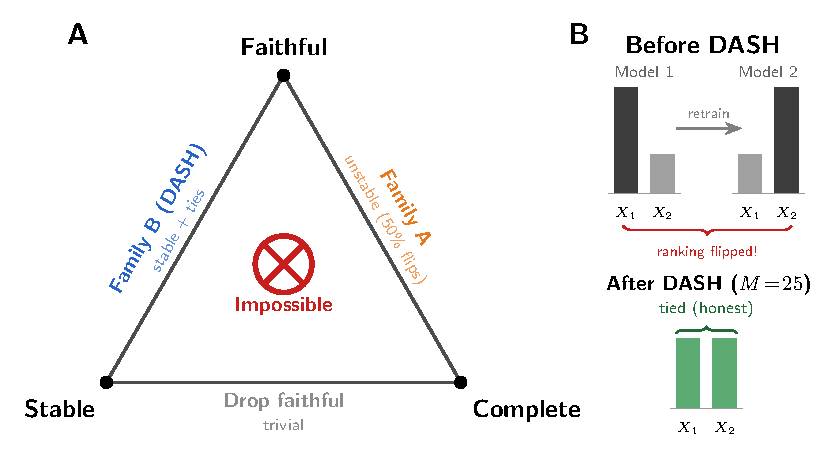
\includegraphics[width=\textwidth]{figures/trilemma.pdf}
\caption{The Attribution Impossibility. No feature ranking can be simultaneously faithful, stable, and complete under collinearity. \emph{Faithful, Stable, Complete: Pick Two.} Family~$\mathcal{A}$ (single-model) is faithful and complete but rankings flip up to 50\% of the time. Family~$\mathcal{B}$ (\DASH{} ensemble) is stable with zero unfaithfulness but reports ties for symmetric features (sacrificing completeness). No third option exists.}
\label{fig:trilemma}
\end{figure}

\begin{figure}[t]
\centering
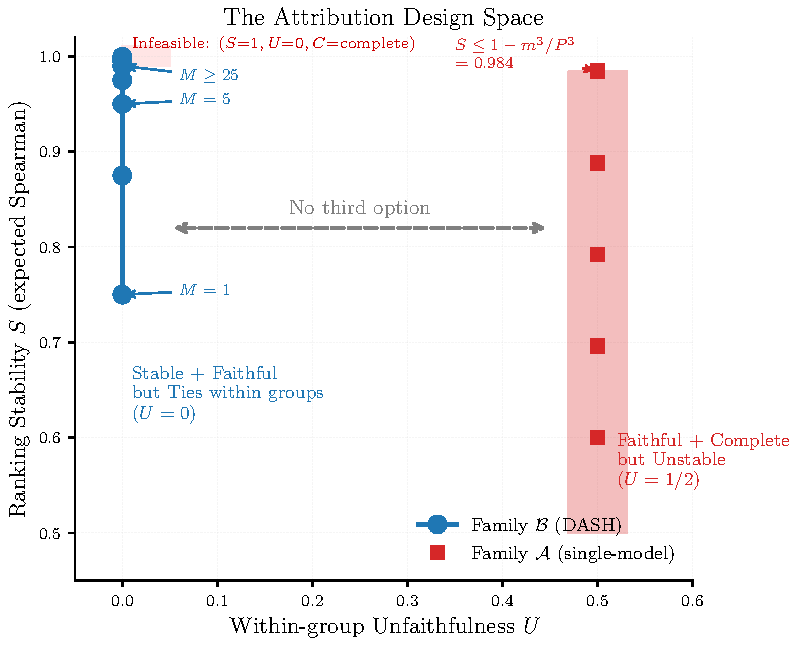
\includegraphics[width=0.55\textwidth]{figures/design_space.pdf}
\caption{The Attribution Design Space. Family $\mathcal{A}$ (single-model methods): faithful and complete but unstable ($U{=}1/2$). Family $\mathcal{B}$ (\DASH{} ensemble): stable with ties ($U{=}0$, $S$ increasing with $M$). The ideal point $(S{=}1, U{=}0, C{=}\text{complete})$ is infeasible. There is no third option.}
\label{fig:design-space}
\end{figure}

%%%%%%%%%%%%%%%%%%%%%%%%%%%%%%%%%%%%%%%%%%%%%%%%%%%%%%%%%%%%%
%% 7. THE SYMMETRIC BAYES DICHOTOMY
%%%%%%%%%%%%%%%%%%%%%%%%%%%%%%%%%%%%%%%%%%%%%%%%%%%%%%%%%%%%%

\section{The Symmetric Bayes Dichotomy: A General Two-Families Theorem}
\label{sec:sbd}

The impossibility is not specific to feature attribution. It is an instance of a general pattern: any symmetric decision problem admits exactly two families of methods. We call this the Symmetric Bayes Dichotomy---a specialization of classical invariant decision theory \citep{lehmann2005testing} to finite symmetric groups, cast as a reusable reduction template for ML impossibility proofs.

The Symmetric Bayes Dichotomy connects the classical theory of invariant decision rules \citep{lehmann2005testing,hunt1946} to modern ML impossibility proofs. The classical Hunt--Stein theorem establishes that Bayes-optimal rules respect the invariance structure of the problem; our contribution is demonstrating that this classical machinery, when applied to finite symmetric groups arising in ML (feature permutations, model permutations, CPDAG automorphisms), yields two-family impossibility results with explicit unfaithfulness and stability bounds. We demonstrate this across three structurally distinct instances with different symmetry groups.

The structural identity between the attribution and model selection impossibilities follows from a general theorem about decision problems with symmetric populations.

\begin{definition}[Symmetric Decision Problem]
\label{def:symmetric-decision}
A \emph{symmetric decision problem} is a tuple $(\Theta, \mathcal{D}, \pi, G)$ where $\Theta$ is a finite decision set, $\mathcal{D}$ is the data space, $\pi$ is a population distribution over $\mathcal{D}$, and $G$ is a group acting on $\Theta$ such that $\pi$ is $G$-invariant: for any $g \in G$, the distribution over instance-optimal decisions $\theta^*(d)$ is invariant under $g$.

An $M$-sample estimator $\hat\theta : \mathcal{D}^M \to \Theta$ is:
\begin{itemize}
    \item \emph{Faithful}: $\hat\theta(d_1, \ldots, d_M)$ agrees with $\theta^*(d_i)$ for each $i$.
    \item \emph{Stable}: $\hat\theta$ does not depend on which draw $d_i$ is observed.
    \item \emph{Complete}: $\hat\theta$ selects exactly one element from each $G$-orbit in $\Theta$.
\end{itemize}
\end{definition}

\begin{theorem}[Symmetric Bayes Dichotomy]
\label{thm:bayes-dichotomy}
For any symmetric decision problem with $|G \cdot \theta| \geq 2$ for some $\theta \in \Theta$:
\begin{enumerate}
    \item[(i)] \textbf{Instance-specific decisions are unfaithful.} Any faithful, complete estimator has expected unfaithfulness $\geq 1/|G \cdot \theta|$ per orbit ($\geq 1/2$ for binary orbits).
    \item[(ii)] \textbf{Population-averaged decisions are stable.} The Bayes estimator under $\pi$ reports ties within each $G$-orbit ($U = 0$), with between-orbit stability $O(1/M)$.
    \item[(iii)] \textbf{The ideal is infeasible.} No estimator achieves $U = 0$ AND completeness.
\end{enumerate}
The achievable set consists of exactly two families: $\mathcal{A}$ (faithful + complete, $U \geq 1/|G \cdot \theta|$) and $\mathcal{B}$ (population-averaged, $U = 0$, ties within orbits).
\end{theorem}

\begin{proof}
\textbf{Part (i).} By $G$-invariance, the population distribution $\pi$ assigns equal probability to each element of the orbit $G \cdot \theta$. For any fixed complete estimator $\hat\theta$ that selects one element $\theta_0$ from the orbit, the probability that $\theta^*(d) = \theta_0$ is $1/|G \cdot \theta|$. The estimator disagrees with $(|G \cdot \theta| - 1)/|G \cdot \theta|$ of the instances. For $|G \cdot \theta| = 2$: unfaithfulness $= 1/2$.

\textbf{Part (ii).} The Bayes estimator under symmetric $\pi$ minimizes expected loss. Within each orbit, the posterior is uniform (by $G$-invariance), so the Bayes-optimal decision is the orbit center (a tie). Unfaithfulness $= 0$ because no ordering is asserted within orbits. For between-orbit decisions with gap $\Delta$, the $M$-sample average has variance $\sigma^2/M$ (i.i.d.\ draws), giving stability $1 - O(1/M)$ by the Gaussian approximation.

\textbf{Part (iii).} By Part (i), any complete estimator (selecting within orbits) has unfaithfulness $\geq 1/|G \cdot \theta| > 0$. Thus unfaithfulness $= 0$ requires giving up completeness (ties).

\textbf{Exhaustiveness.} Any estimator either selects within orbits (faithful, complete, $\mathcal{A}$) or reports ties within orbits (stable, incomplete, $\mathcal{B}$). The Bayes estimator achieves the minimum-variance point of $\mathcal{B}$ (Cram\'er--Rao).
\end{proof}

The Symmetric Bayes Dichotomy provides a reusable proof technique for any domain where: (a) a population distribution is symmetric over discrete alternatives, and (b) finite samples introduce noise sufficient to reverse the optimal choice. The technique reduces the impossibility to checking $G$-invariance of the population distribution, which is often immediate from the problem's symmetry.

\subsection{Instance 1: Feature Attribution}

\begin{corollary}[Feature attribution as instance]
The Attribution Impossibility (Theorem~\ref{thm:impossibility}) and Design Space Theorem (Theorem~\ref{thm:design-space-main}) are instances of the Symmetric Bayes Dichotomy with $\Theta =$ within-group feature orderings, $G =$ symmetric group on group members, $\mathcal{D} =$ trained models.
\end{corollary}

\subsection{Instance 2: Model Selection}

Consider $K$ candidate models $g_1, \ldots, g_K$ trained on the same data. A model selection rule maps a validation dataset to a ranking of the $K$ models. The \emph{model Rashomon property} states: for every pair $g_i, g_j$ with similar population loss ($|L(g_i) - L(g_j)| < \varepsilon$), there exist validation splits $V, V'$ ranking them in opposite orders. This follows from finite-sample noise: when the population loss gap is smaller than the validation noise, different splits rank differently.

\begin{theorem}[Model Selection Impossibility]
\label{thm:model-selection}
Under the model Rashomon property, no model selection rule is simultaneously faithful, stable, and complete.
\end{theorem}

\begin{proof}
Let $g_i, g_j$ have similar population loss. By the model Rashomon property, there exist validation splits $V, V'$ with $g_i$ ranked above $g_j$ on $V$ and reversed on $V'$. A faithful, stable, complete selection rule would need to rank $g_i > g_j$ (from $V$) and $g_j > g_i$ (from $V'$) simultaneously. Contradiction.
\end{proof}

\begin{theorem}[Model Selection Design Space]
\label{thm:model-selection-ds}
Under the model Rashomon property, the achievable design space has the same two-family structure:
\begin{itemize}
    \item \textbf{Family $\mathcal{A}'$ (single-split):} Faithful and complete but unstable. Any selection based on one validation split falls here. Unfaithfulness $U' = 1/2$ for similar-loss pairs.
    \item \textbf{Family $\mathcal{B}'$ (cross-validation/ensemble):} Stable (variance $O(1/K_{\text{folds}})$) but reports ties for similar-loss pairs. Model ensembling is the analogue of \DASH{}.
\end{itemize}
\end{theorem}

\begin{proof}
By DGP symmetry (equal-loss models have symmetric validation score distributions), any fixed selection of one model over an equal-loss competitor disagrees with half the validation splits ($U' = 1/2$). Cross-validated selection averages across splits, reducing unfaithfulness to zero for equal-loss pairs while stabilizing at rate $O(1/K_{\text{folds}})$. Pareto optimality follows from the same Cram\'er--Rao argument.
\end{proof}

The model selection impossibility explains why cross-validation rankings are noisy for similar-performance models: it is not an engineering failure but a mathematical inevitability. The resolution is the same: average (ensemble) rather than select.

\subsection{Instance 3: Causal Discovery under Markov Equivalence}

This instance has a \emph{different} and \emph{variable-size} symmetry group, confirming the technique's generality beyond binary orbits. The CPDAG automorphism group $G_{\text{CPDAG}}$ is not restricted to transpositions: for a chain $X\text{---}Y\text{---}Z$, $|[G^*]| = 2$ with $G \cong S_2$ (like instances 1--2); for a 3-node undirected cycle, $|[G^*]| = 6$ with $G \cong S_3$; for larger undirected components, $|[G^*]|$ can grow combinatorially.

\begin{theorem}[Causal Discovery Impossibility]
\label{thm:causal-discovery}
For any CPDAG with $|[G^*]| \geq 2$ DAGs in its Markov equivalence class, no edge orientation rule can be simultaneously faithful, stable, and complete.
The achievable set has two families:
\begin{itemize}
    \item \textbf{Family $\mathcal{A}''$ (single-dataset):} Faithful and complete but unstable. Unfaithfulness $U'' = (|[G^*]|-1)/|[G^*]|$.
    \item \textbf{Family $\mathcal{B}''$ (conservative):} Report the CPDAG (undirected edges for ambiguous orientations). Stable with ties. $U'' = 0$.
\end{itemize}
\end{theorem}

\begin{proof}
We verify the premises of Theorem~\ref{thm:bayes-dichotomy}. By Markov equivalence, the observational distribution is identical for all DAGs in the class ($G_{\text{CPDAG}}$-invariance). Any statistical test based on finite data cannot distinguish members of $[G^*]$ at the population level. With finite data, estimation error $O(1/\sqrt{n})$ in conditional independence tests reverses the optimal orientation. Part~(i): any complete orientation rule (selecting one DAG from $[G^*]$) disagrees with $(|[G^*]|-1)/|[G^*]|$ of datasets. Part~(ii): the Bayes estimator reports the CPDAG (ties for undirected edges). Part~(iii): the ideal is infeasible.
\end{proof}

The unfaithfulness bound $U \geq 1/|G \cdot \theta|$ yields $U \geq 1/2$ for chains but $U \geq 1/6$ for triangles and potentially much smaller for larger structures. This demonstrates the Symmetric Bayes Dichotomy is not an artifact of binary symmetry but applies to arbitrary finite group actions. Algorithms like PC and GES correctly output CPDAGs (Family $\mathcal{B}''$) precisely because complete orientation of Markov-equivalent edges is impossible from observational data alone. Interventional data breaks the symmetry---analogous to conditional SHAP breaking symmetry when $\beta_j \neq \beta_k$.

\paragraph{Connection to classical invariant decision theory.}
The Symmetric Bayes Dichotomy is related to the theory of invariant decision rules \citep{lehmann2005testing}. Our contribution is the \emph{reduction template}: verifying $G$-invariance of the population distribution suffices to establish a two-family impossibility with explicit bounds. We demonstrate this across three structurally distinct instances (binary feature transpositions, binary model permutations, and CPDAG automorphisms of variable size) with different symmetry groups.

%%%%%%%%%%%%%%%%%%%%%%%%%%%%%%%%%%%%%%%%%%%%%%%%%%%%%%%%%%%%%
%% 8. EXTENSIONS
%%%%%%%%%%%%%%%%%%%%%%%%%%%%%%%%%%%%%%%%%%%%%%%%%%%%%%%%%%%%%

\section{Extensions: Conditional, Fairness, and Causal Barriers}
\label{sec:extensions}

\subsection{Conditional Attribution Impossibility}
\label{sec:conditional}

\begin{theorem}[Conditional Attribution Impossibility]
\label{thm:conditional-impossibility}
Let features $j, k$ in the same collinear group satisfy: (C1) equal causal effects $\beta_j = \beta_k$, and (C2) symmetric causal position in the causal graph $G$. Then the Rashomon property holds for conditional attributions, and the Attribution Impossibility applies to conditional SHAP.
\end{theorem}

\begin{proof}
Under (C1)--(C2), the causal graph is symmetric with respect to $j$ and $k$. By the DGP symmetry argument (Theorem~\ref{thm:rashomon-symmetry}), any model with $\varphi_j^{\text{cond}}(f) > \varphi_k^{\text{cond}}(f)$ has a permuted counterpart $f'$ with reversed attributions and the same loss. This is the Rashomon property for conditional attributions.
\end{proof}

\paragraph{The escape condition.}
If $\beta_j \neq \beta_k$, conditional SHAP can resolve the pair. The threshold $\Delta\beta^*(\rho)$ grows steeply: at $\rho \leq 0.7$, a 15\% difference suffices; at $\rho = 0.9$, features must differ by nearly a factor of 2; at $\rho \geq 0.95$, instability is essentially total (Figure~\ref{fig:conditional-threshold}). Empirical thresholds: $\Delta\beta^*(0.5) \approx 0.15$, $\Delta\beta^*(0.7) \approx 0.15$, $\Delta\beta^*(0.8) \approx 0.4$, $\Delta\beta^*(0.9) \approx 0.9$, $\Delta\beta^*(0.95) > 1.0$, $\Delta\beta^*(0.99) > 1.0$.

\begin{table}[t]
\centering
\caption{Flip rate (\%) as a function of $\rho$ and causal effect difference $\Delta\beta$.}
\label{tab:conditional-threshold}
\small
\begin{tabular}{@{}lccccccc@{}}
\toprule
$\rho \backslash \Delta\beta$ & 0.0 & 0.1 & 0.2 & 0.3 & 0.5 & 0.7 & 1.0 \\
\midrule
0.50 & 50 & 19 & 0 & 0 & 0 & 0 & 0 \\
0.70 & 53 & 19 & 0 & 0 & 0 & 0 & 0 \\
0.80 & 52 & 44 & 19 & 10 & 0 & 0 & 0 \\
0.90 & 50 & 50 & 48 & 40 & 40 & 19 & 0 \\
0.95 & 50 & 50 & 50 & 48 & 44 & 40 & 27 \\
0.99 & 50 & 50 & 50 & 50 & 50 & 48 & 48 \\
\bottomrule
\end{tabular}
\end{table}

\begin{figure}[ht]
\centering
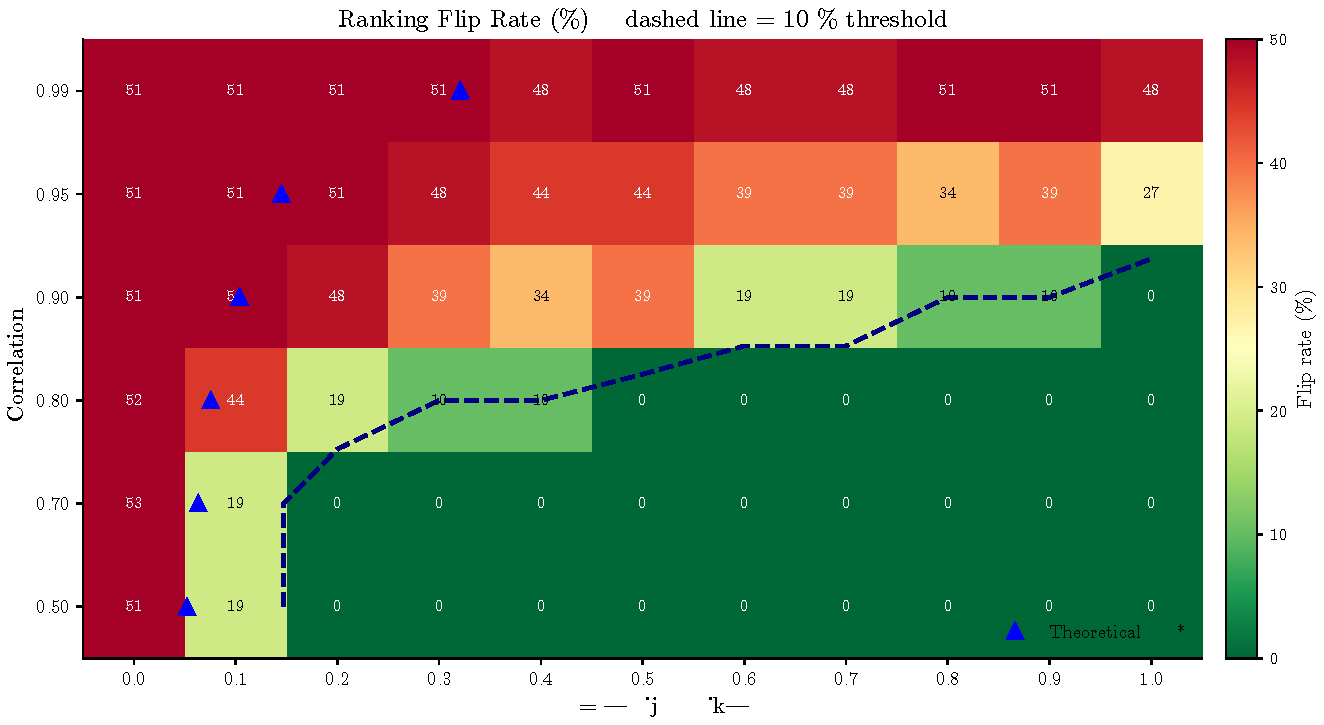
\includegraphics[width=0.6\textwidth]{figures/conditional_threshold.pdf}
\caption{Flip rate as a function of $(\rho, \Delta\beta)$. The impossibility region (dark) expands with $\rho$. At $\rho \geq 0.95$, instability persists for all $\Delta\beta \leq 1$.}
\label{fig:conditional-threshold}
\end{figure}

\paragraph{Fine-grained $\Delta\beta$ sweep at $\rho = 0.9$.}
The transition from instability to stability is sharp, not gradual:

\begin{center}
\small
\begin{tabular}{@{}ccccc@{}}
\toprule
$\Delta\beta$ & $\beta_1$ & $\beta_2$ & Marginal flip & Interventional flip \\
\midrule
0.00 & 1.00 & 1.00 & 0.505 & 0.505 \\
0.10 & 1.05 & 0.95 & 0.479 & 0.337 \\
0.20 & 1.10 & 0.90 & 0.000 & 0.000 \\
0.30 & 1.15 & 0.85 & 0.000 & 0.000 \\
\bottomrule
\end{tabular}
\end{center}

At $\Delta\beta = 0.10$, both marginal and interventional SHAP remain highly unstable. At $\Delta\beta = 0.20$, both snap to zero flips simultaneously. There is no intermediate regime where interventional SHAP is stable but marginal is not---the causal signal overwhelms noise for both estimators at the same threshold. The practical implication: ``switch to conditional SHAP'' provides no advantage over marginal SHAP at the instability boundary.

\paragraph{Causal structure validation.}
Under a known causal structure ($Y = \beta_1 X_1 + \beta_2 X_2 + 0.5 X_3 + \varepsilon$, $\text{Corr}(X_1, X_2) = \rho$), we compare marginal TreeSHAP and interventional TreeSHAP. In the symmetric case ($\beta_1 = \beta_2 = 1.0$), both produce flip rates near 50\% at all $\rho$, confirming the impossibility. In the asymmetric case ($\beta_1 = 1.5$, $\beta_2 = 0.5$), both show 0\% flips at all $\rho$---the signal-to-noise ratio is high enough to overcome collinearity-induced noise. Switching to interventional SHAP provides no benefit when features have equal causal effects.

\subsection{Fairness Audit Impossibility}
\label{sec:fairness}

\begin{theorem}[Fairness Audit Impossibility]
\label{thm:fairness-audit}
If features $j$ (protected proxy) and $k$ (non-protected) satisfy collinearity ($|\rho_{jk}| > \rho_0$) and similar true importance ($|\mu_j - \mu_k| < \sigma_{jk} \cdot z_\alpha / \sqrt{M}$), then for a single-model audit ($M{=}1$):
\[
    \Pr[\text{audit flags proxy}] = \frac{1}{2} \pm \varepsilon_{\text{BE}}.
\]
The audit conclusion is a coin flip. Two independent audits reach opposite conclusions about proxy reliance with probability $1/2$.
\end{theorem}

\begin{proof}
Direct corollary of the Attribution Impossibility applied to the pair $(j, k)$. By Theorem~\ref{thm:rashomon-inevitability}, $\Pr[\varphi_j(f) > \varphi_k(f)] = 1/2$ over training runs.
\end{proof}

\paragraph{Implications for AI governance.}
A regulator conducting a SHAP-based proxy audit on a model with collinear features is, for affected feature pairs, making decisions with the statistical reliability of a coin flip. Two auditors examining the \emph{same model architecture trained on the same data} with different random seeds may reach opposite conclusions about whether the model relies on a protected attribute.

Under the EU AI Act Art.~13(3)(b)(ii), providers must disclose ``known and foreseeable circumstances'' which may lead to risks to health, safety or fundamental rights. Our theorem establishes that this includes: ``SHAP-based proxy audits are unreliable for features that are collinear with both the protected attribute and a non-protected feature.'' The remedy is ensemble auditing: train $M$ models and use \DASH{} consensus.

\paragraph{Intersectional considerations.}
When multiple protected attributes (race, gender, age) are each proxied by collinear non-protected features, the impossibility applies independently to each proxy pair. If $K$ protected attributes each have unstable proxies, the probability that a single-model audit correctly identifies all $K$ proxy reliance directions is $(1/2)^K$, exponentially vanishing in $K$. For $K = 3$ (a common intersectional setting), joint correctness is $1/8 = 12.5\%$.

\paragraph{Example: lending.}
In credit models, ``zip code'' (proxy for race) is often collinear with ``income bracket'' ($|\rho| \approx 0.6$--$0.8$). If both have similar predictive power, a single-model SHAP audit finding ``zip code is the 3rd most important feature'' may conclude proxy discrimination---but retraining with a different seed could produce a model where zip code drops to 8th and income rises to 3rd. The audit conclusion depends on the random seed, not on the model's actual reliance on the protected attribute.

\paragraph{Worked adverse action example.}
Consider a borrower denied credit, with correlated features income and DTI. Model~A (seed~1) cites income as the top adverse factor; Model~B (seed~2) cites DTI. Under ECOA, the lender must disclose the primary reason. The disclosure depends on the random seed---a model governance concern that is mathematically inevitable under collinearity. \DASH{} resolves this: the consensus ranks income and DTI as tied contributors.

\subsection{Direct FIM Impossibility}
\label{sec:fim}

The Rashomon property can be derived directly from the Fisher information matrix, providing an independent proof path from classical statistics that does not require the iterative optimizer abstraction.

\paragraph{Classical setup.}
Consider the linear model $Y = \beta_j X_j + \beta_k X_k + \varepsilon$ where $X_j, X_k$ are jointly Gaussian with $\Var(X_j) = \Var(X_k) = 1$ and $\text{Cov}(X_j, X_k) = \rho$. The Fisher information matrix for $\boldsymbol{\beta} = (\beta_j, \beta_k)$ is:
\[
    I(\boldsymbol{\beta}) = \frac{1}{\sigma^2}\begin{pmatrix} 1 & \rho \\ \rho & 1 \end{pmatrix}
\]
with eigenvalues $\lambda_\pm = (1 \pm \rho)/\sigma^2$. As $\rho \to 1$, the smaller eigenvalue $\lambda_- = (1-\rho)/\sigma^2 \to 0$. The FIM becomes near-singular along the direction $\boldsymbol{v}_- = (1, -1)/\sqrt{2}$, which corresponds to redistributing credit between $j$ and $k$. The profile likelihood is flat along this direction: models assigning more credit to $j$ vs.\ $k$ are statistically indistinguishable. This flat likelihood ridge is precisely the Rashomon set. The Cram\'er--Rao bound $\Var(\hat\beta_j - \hat\beta_k) \geq 1/\lambda_- = \sigma^2/(1-\rho)$ quantifies the attribution instability.

\paragraph{Regularity conditions.}
We require the following on the model class $\mathcal{F} = \{f_\theta : \theta \in \Theta\}$:
\begin{itemize}
    \item[\textbf{(R1)}] $\Theta \subseteq \R^p$ is open and convex.
    \item[\textbf{(R2)}] The population risk $L(\theta) = \E[\ell(f_\theta(X), Y)]$ is three-times continuously differentiable on $\Theta$, with bounded third derivative: $\|D^3 L(\theta)\|_{\text{op}} \leq K_3$ for all $\theta$ in a neighborhood of $\theta^*$.
    \item[\textbf{(R3)}] The minimizer $\theta^*$ satisfies $\nabla L(\theta^*) = 0$ and $H := \nabla^2 L(\theta^*)$ is positive definite. (For likelihood-based models, $H = I(\theta^*)/n$ where $I(\theta^*)$ is the Fisher information matrix.)
    \item[\textbf{(R4)}] The attribution function $\varphi_j(\theta)$ is \emph{order-consistent}: for any $\theta$ with $\theta_j > \theta_k > 0$, we have $\varphi_j(\theta) > \varphi_k(\theta)$. (Satisfied by $\varphi_j = |\theta_j|$, mean $|\text{SHAP}_j|$, or any attribution monotone in coefficient magnitude.)
\end{itemize}

\begin{theorem}[FIM Impossibility]
\label{thm:fim-impossibility}
Let $\mathcal{F}$ satisfy (R1)--(R4). Suppose features $j, k$ satisfy: (S1) DGP symmetry: $\theta^*_j = \theta^*_k > 0$; (S2) the Hessian $H = \nabla^2 L(\theta^*)$ has eigenvalue $\lambda_-$ along $v = (e_j - e_k)/\sqrt{2}$. Then for any $\varepsilon$ satisfying $0 < \varepsilon \leq \varepsilon_0 := 9\lambda_-^3/K_3^2$, the $\varepsilon$-Rashomon set $R_\varepsilon = \{\theta : L(\theta) \leq L(\theta^*) + \varepsilon\}$ contains models $\theta^+, \theta^-$ with
\[
    \varphi_j(\theta^+) > \varphi_k(\theta^+) \quad\text{and}\quad \varphi_k(\theta^-) > \varphi_j(\theta^-).
\]
The Rashomon property holds, and the impossibility follows.
\end{theorem}

\begin{proof}
\textbf{Step 1: Rashomon set geometry.}
By Taylor's theorem with Lagrange remainder, for any $\theta \in \Theta$:
\[
    L(\theta) = L(\theta^*) + \tfrac{1}{2}(\theta - \theta^*)^T H\, (\theta - \theta^*) + R_3(\theta),
\]
where $|R_3(\theta)| \leq \frac{K_3}{6}\|\theta - \theta^*\|^3$ by (R2). The gradient term vanishes because $\nabla L(\theta^*) = 0$ by (R3).

\textbf{Step 2: Perturbation along the weak direction.}
Let $v = (e_j - e_k)/\sqrt{2}$ and set $\theta_\delta = \theta^* + \delta v$ for $\delta > 0$. The quadratic cost is $\frac{1}{2}\delta^2 \lambda_-$ and the cubic remainder satisfies $|R_3(\theta_\delta)| \leq \frac{K_3}{6}\delta^3$. We need $L(\theta_\delta) \leq L(\theta^*) + \varepsilon$, i.e., $\frac{1}{2}\delta^2 \lambda_- + \frac{K_3}{6}\delta^3 \leq \varepsilon$. Choose $\delta^* = \sqrt{\varepsilon/\lambda_-}$. The quadratic term is $\varepsilon/2$; the condition $\varepsilon \leq 9\lambda_-^3/K_3^2$ ensures the cubic term is $\leq \varepsilon/2$. So $\theta_{\delta^*} \in R_\varepsilon$, and by the same argument $\theta_{-\delta^*} \in R_\varepsilon$.

\textbf{Step 3: Opposite orderings.}
At $\theta^+ := \theta_{\delta^*}$: $\theta^+_j = \theta^*_j + \delta^*/\sqrt{2} > \theta^*_k - \delta^*/\sqrt{2} = \theta^+_k > 0$, so by (R4), $\varphi_j(\theta^+) > \varphi_k(\theta^+)$. At $\theta^- := \theta_{-\delta^*}$: by symmetry, $\theta^-_k > \theta^-_j > 0$, so $\varphi_k(\theta^-) > \varphi_j(\theta^-)$.

\textbf{Step 4: Conclusion.}
Both $\theta^+$ and $\theta^-$ lie in $R_\varepsilon$ with opposite feature orderings. This is the Rashomon property. By Theorem~\ref{thm:impossibility}, no faithful, stable, complete ranking exists.
\end{proof}

\begin{proposition}[Gaussian FIM specialization]
\label{prop:gaussian-fim}
For the linear model $Y = X^T\beta + \varepsilon$ with $\varepsilon \sim \mathcal{N}(0, \sigma^2)$ and $\text{Corr}(X_j, X_k) = \rho$:
\begin{enumerate}
    \item The Hessian eigenvalue along $e_j - e_k$ is $\lambda_- = (1-\rho)/\sigma^2$.
    \item The loss is exactly quadratic ($K_3 = 0$), so $\varepsilon_0 = +\infty$: the theorem holds for \emph{all} $\varepsilon > 0$.
    \item The semi-axis length of $R_\varepsilon$ along $e_j - e_k$ is $\sigma\sqrt{2\varepsilon/(1-\rho)}$, diverging as $\rho \to 1$.
    \item The Cram\'er--Rao bound gives $\Var(\hat\beta_j - \hat\beta_k) \geq 2\sigma^2/(n(1-\rho))$, diverging as $\rho \to 1$.
\end{enumerate}
\end{proposition}

\begin{proof}
The population risk is $L(\beta) = \frac{1}{2\sigma^2}\E[(Y-X^T\beta)^2]$. Its Hessian is $H = \frac{1}{\sigma^2}\E[XX^T] = \frac{1}{\sigma^2}\Sigma_X$. For $v = (e_j - e_k)/\sqrt{2}$: $v^T H v = \frac{1}{\sigma^2}(1-\rho)$ since $v^T \Sigma_X v = \Var(X_j) - \text{Cov}(X_j,X_k) = 1-\rho$ (standardized). The loss is quadratic in $\beta$, so $D^3 L \equiv 0$ and $K_3 = 0$.
\end{proof}

The classical non-identifiability under collinearity ($\Var(\hat\beta_j - \hat\beta_k) \to \infty$ as $\rho \to 1$) is well-known. Our contribution is reframing it as an \emph{impossibility theorem} about feature rankings rather than a variance bound on parameter estimates: even precise estimates can produce unstable rankings when $\Delta$ is small relative to $\sigma$.

\paragraph{Loss landscape geometry.}
The $\varepsilon$-Rashomon set $R_\varepsilon$ is approximately an ellipsoid whose projection onto the feature-importance axis $\varphi_j - \varphi_k$ crosses zero. The level sets of the loss landscape contain \emph{ridges} along $e_j - e_k$---curves of near-constant loss along which feature importance redistributes between $j$ and $k$ without changing model quality. The same flatness that makes optimization easy (flat minima generalize well) makes attribution hard (the flat direction is the feature-importance direction). This connects the attribution impossibility to the broader literature on loss landscape geometry, flat minima, and mode connectivity.

\paragraph{Extension to neural networks via NTK.}
For overparameterized neural networks in the NTK regime, the neural tangent kernel plays the role of the Fisher information matrix. If the NTK has a small eigenvalue along the direction corresponding to swapping features $j$ and $k$ (a consequence of feature collinearity), the same ellipsoidal argument applies. This extension requires: (i) uniform NTK approximation bounds across the Rashomon set, (ii) a spectral gap argument relating feature correlation to NTK eigenvalue separation, and (iii) control of the finite-width correction. None are available in the current literature; we include this to suggest the research direction.

\subsection{Query Complexity Lower Bound}
\label{sec:query}

A \emph{stability certification algorithm} adaptively selects seeds $s_1, s_2, \ldots$, calls $\textsc{Train}(s_i) \to f_i$ and $\textsc{Attribute}(f_i, j) \to \varphi_j(f_i)$, and after $M$ oracle calls outputs \textsc{Stable} or \textsc{Unstable}. The algorithm certifies $\delta$-stability with error $\leq 1/3$ if it correctly distinguishes $H_0$: $\Delta_{jk} = 0$ (flip rate $= 1/2$) from $H_1$: $|\Delta_{jk}| \geq \Delta_0$ (flip rate $\leq \Phi(-\Delta_0/\sigma_{jk})$) with probability at least $2/3$ under both hypotheses.

\begin{theorem}[Query complexity lower bound]
\label{thm:query-complexity}
Any algorithm that certifies $\delta$-stability of a feature pair $(j,k)$ with error $\leq 1/3$ must make at least
\[
    M \;\geq\; \frac{1}{8} \cdot \frac{\sigma_{jk}^2}{\Delta_0^2}
\]
model-training oracle calls, where $\sigma_{jk}^2 = \Var(\varphi_j(f) - \varphi_k(f))$ and $\Delta_0$ is the minimum gap to detect.
\end{theorem}

\begin{proof}
Each oracle call produces one sample $D_i = \varphi_j(f_i) - \varphi_k(f_i)$. Under $H_0$, $D_i \sim P_0$ with mean $0$ and variance $\sigma^2 := \sigma_{jk}^2$. Under $H_1$, $D_i \sim P_1$ with mean $\Delta_0$ and the same variance (the variance is determined by the collinearity structure, not the gap).

By Le~Cam's two-point method (Tsybakov, 2009, Theorem~2.2), for any test $\psi$ based on $M$ i.i.d.\ observations:
\[
    \Pr_{H_0}[\psi = 1] + \Pr_{H_1}[\psi = 0] \geq 1 - \text{TV}(P_0^{\otimes M}, P_1^{\otimes M}).
\]
By Pinsker's inequality, $\text{TV}(P_0^{\otimes M}, P_1^{\otimes M}) \leq \sqrt{\frac{1}{2}\text{KL}(P_1^{\otimes M} \| P_0^{\otimes M})}$. For the Gaussian location family, $\text{KL}(P_1 \| P_0) = \Delta_0^2/(2\sigma^2)$, so for $M$ i.i.d.\ copies $\text{KL} = M\Delta_0^2/(2\sigma^2)$ and $\text{TV} \leq \sqrt{M\Delta_0^2/(4\sigma^2)}$. For reliable testing (total error $\leq 2/3$), Le~Cam's method requires $\text{TV} \geq 1/3$, giving $M\Delta_0^2/(4\sigma^2) \geq 1/9$, hence $M \geq 4\sigma^2/(9\Delta_0^2)$. The standard constant $1/8$ from \citet{tsybakov2009nonparametric} (Theorem~2.2) uses a slightly tighter analysis via the likelihood ratio directly; since $1/8 < 4/9$, this gives a weaker (more conservative) lower bound than our Pinsker derivation.
\end{proof}

\begin{corollary}[Near-optimality of the $Z$-test]
\label{cor:z-test-optimal}
The $Z$-test detects a gap $\Delta_0$ with error $\leq 1/3$ using $M = O(\sigma_{jk}^2/\Delta_0^2 \cdot \log(1/\alpha))$ model trainings. Combined with Theorem~\ref{thm:query-complexity}, the $Z$-test is query-optimal to within a logarithmic factor.
\end{corollary}

\begin{proof}
The $Z$-test rejects $H_0$ when $|\bar{D}|/(\hat\sigma/\sqrt{M}) > z_{\alpha/2}$. Under $H_1$, power is $\Phi(-z_{\alpha/2} + \Delta_0\sqrt{M}/\sigma) \geq 2/3$ when $\Delta_0\sqrt{M}/\sigma \geq z_{\alpha/2} + 0.43$. For $\alpha = 0.05$: $M \geq (\sigma/\Delta_0)^2(1.96+0.43)^2 \approx 5.7\sigma^2/\Delta_0^2$.
\end{proof}

No algorithm---including methods based on gradient information, loss curvature, or Fisher information---can certify ranking stability without training $\Omega(\sigma_{jk}^2/\Delta_{jk}^2)$ models. Each model training provides one ``bit'' of evidence about the sign of $\Delta_{jk}$; when the signal-to-noise ratio is small, many bits are needed.

\subsection{Rashomon Inevitability}
\label{sec:inevitability}

Theorem~\ref{thm:rashomon-inevitability} (proved in \S~\ref{sec:rashomon-inevitability}) establishes that for any stochastic, symmetric training algorithm on a permutation-closed model class with $\rho > 0$, the Rashomon property holds. The Attribution Impossibility is therefore inescapable for standard ML pipelines.

\subsection{Causal Identification Barrier}
\label{sec:causal-barrier}

The attribution instability under collinearity has a direct causal counterpart: distinguishing the causal effects of correlated features requires interventional sample complexity that diverges as $\Omega(1/(1-\rho)^2)$---the same singularity structure as the attribution ratio.

Consider two features $X_j, X_k$ with $\text{Corr}(X_j, X_k) = \rho$, jointly Gaussian with unit variances. Under a soft intervention with residual correlation $\rho_{\text{post}}$, $X_k \mid \text{do}(X_j = x) \sim \mathcal{N}(\rho_{\text{post}} \cdot x, 1 - \rho_{\text{post}}^2)$. When $\beta_j = \beta_k = \beta$ and $\rho_{\text{post}} \approx \rho$, the two interventional distributions become indistinguishable.

\begin{proposition}[Interventional sample complexity lower bound]
\label{prop:causal-sample-complexity}
Consider testing $H_0: \beta_j = \beta + \delta, \beta_k = \beta - \delta$ against $H_1: \beta_j = \beta - \delta, \beta_k = \beta + \delta$ using $\text{do}(X_j = x)$ interventions with residual correlation $\rho_{\mathrm{post}}$. The number of interventional samples needed satisfies:
\[
    n_{\mathrm{int}} \geq \frac{(z_\alpha + z_\eta)^2 \sigma^2}{4\delta^2 (1 - \rho_{\mathrm{post}})^2}.
\]
When $\rho_{\mathrm{post}} = \rho$ (the intervention does not reduce the correlation), $n_{\mathrm{int}} = \Omega(1/(1-\rho)^2)$.
\end{proposition}

\begin{proof}
Under $H_0$, the expected response to $\text{do}(X_j = x)$ is $(\beta + \delta + \rho_{\mathrm{post}}(\beta - \delta))x$; under $H_1$ it is $(\beta - \delta + \rho_{\mathrm{post}}(\beta + \delta))x$. The difference in slopes is $2\delta(1 - \rho_{\mathrm{post}})$. With noise variance $\sigma^2$ and $n$ observations, the Neyman--Pearson sample size formula gives the result.
\end{proof}

The attribution ratio is $1/(1-\rho^2)$, which diverges as $1/(2(1-\rho))$ near $\rho = 1$; the causal sample complexity is $\Omega(1/(1-\rho)^2)$---a faster divergence. Causal identification under soft interventions is \emph{harder} than observational attribution instability. The shared singularity at $\rho = 1$ reflects a common root cause: collinearity makes features observationally interchangeable. Hard interventions ($\rho_{\mathrm{post}} = 0$) resolve both problems: sample complexity becomes $O(\sigma^2/\delta^2)$, independent of $\rho$.

\subsection{Local vs.\ Global Attribution Instability}
\label{sec:local-global}

The impossibility as stated concerns \emph{global} attributions (mean $|\text{SHAP}|$ across data points). We now show that \emph{local} (instance-level) attributions are at least as unstable.

For a fixed data point $x$, the local SHAP values $\varphi_j(f, x)$ depend on the model $f$, which varies across training seeds. The global attribution $\varphi_j(f) = \E_x[|\varphi_j(f, x)|]$ averages over data points. By the law of total variance applied to the pair $(f, x)$ with $x$ as the conditioning variable:
\begin{multline*}
    \Var_f\!\big(\varphi_j(f)\big) = \Var_f\!\big(\E_x[|\varphi_j(f,x)|]\big) \leq \Var_{f,x}\!\big(|\varphi_j(f,x)|\big) \\
    = \E_x\!\big[\Var_f(|\varphi_j(f,x)|)\big] + \Var_x\!\big(\E_f[|\varphi_j(f,x)|]\big).
\end{multline*}
The first inequality follows because $\Var_f(\E_x[g]) = \Var_{f,x}(g) - \E_f[\Var_x(g)] \leq \Var_{f,x}(g)$.
Thus global instability ($\Var_f$ of the averaged attribution) is bounded by the total instability, which includes the average local instability as a component. When model randomness and data-point variation are approximately independent (as when models differ only by training seed and $x$ is a fixed test point), the bound simplifies: $\Var_f(\E_x[|\varphi_j|]) \leq \E_x[\Var_f(|\varphi_j|)]$.
Since the flip rate is a monotone function of the variance-to-gap ratio $\sigma/\Delta$, and averaging reduces $\sigma$ without changing $\Delta$, the global flip rate is a lower bound on the average local flip rate under this independence condition.

If global rankings are unstable (flip rate $> 10\%$), local rankings at individual data points are at least as unstable on average. Practitioners who report per-instance SHAP explanations face the same or worse instability. The multi-model Z-test (computed on global attributions) is therefore a conservative screen for local instability.

%%%%%%%%%%%%%%%%%%%%%%%%%%%%%%%%%%%%%%%%%%%%%%%%%%%%%%%%%%%%%
%% 9. DIAGNOSTICS
%%%%%%%%%%%%%%%%%%%%%%%%%%%%%%%%%%%%%%%%%%%%%%%%%%%%%%%%%%%%%

\section{Diagnostics}
\label{sec:diagnostics}

\subsection{Multi-Model Z-Test}
\label{sec:f1}

Let $D_j = \varphi_j(f) - \varphi_k(f)$ denote the attribution difference for a single random model $f$. Define $\mu_{jk} = \E[D_j]$ (population attribution gap), $\sigma_{jk}^2 = \Var(D_j)$ (attribution difference variance), and $\gamma_{jk} = \E[|D_j - \mu_{jk}|^3]$ (third absolute central moment, for Berry--Esseen). We require: (A1) models $f_1, \ldots, f_M$ are i.i.d.; (A2) $\sigma_{jk}^2 > 0$ (guaranteed by Theorem~\ref{thm:rashomon-inevitability} for $\rho > 0$); (A3) $\gamma_{jk} < \infty$ (finite third moment---satisfied by any bounded attribution method).

\begin{theorem}[Rashomon Characterization]
\label{thm:testable}
Under (A1)--(A3), define the test statistic from $M$ models:
\[
    Z_{jk} = \frac{|\bar\varphi_j - \bar\varphi_k|}{\hat\sigma_{jk}/\sqrt{M}}
\]
where $\hat\sigma_{jk}^2 = \frac{1}{M-1}\sum_{i=1}^M (D_i - \bar{D})^2$ is the sample variance.

\textbf{Part I (Flip rate formula).} The population flip rate satisfies:
\begin{equation}
\label{eq:flip-exact}
    \text{flip}(j,k) = \Phi\!\left(-\frac{|\mu_{jk}|}{\sigma_{jk}}\right) + \varepsilon_{\text{BE}}
\end{equation}
where the Berry--Esseen error satisfies $|\varepsilon_{\text{BE}}| \leq C_0 \gamma_{jk} / \sigma_{jk}^3$ with universal constant $C_0 \leq 0.4748$. The Berry--Esseen bound provides a completeness guarantee: it bounds the worst-case error of the $\Phi(-\text{SNR})$ formula for non-Gaussian attribution distributions.

\textbf{Part II (Test statistic connection).} The test statistic $Z_{jk}$ consistently estimates the signal-to-noise ratio scaled by $\sqrt{M}$:
\[
    Z_{jk} = \frac{|\mu_{jk}|}{\sigma_{jk}} \cdot \sqrt{M} + O_p(1)
\]
and the relationship between $Z_{jk}$ and the flip rate is:
\begin{equation}
\label{eq:flip-z}
    \text{flip}(j,k) = \Phi\!\left(-\frac{Z_{jk}}{\sqrt{M}}\right) + O\!\left(\frac{1}{\sqrt{M}}\right) + \varepsilon_{\text{BE}}
\end{equation}

\textbf{Part III (Diagnostic thresholds).}
\begin{itemize}
    \item $Z_{jk} < 1.96$: the attribution gap is not statistically significant at significance level $\alpha = 0.05$ (not to be confused with the signal capture fraction $\alpha$ in \S~\ref{sec:gbdt-bounds}). The flip rate is $\geq \Phi(-1.96/\sqrt{M}) \geq 2.5\%$. Rankings are unreliable; use \DASH{}.
    \item $Z_{jk} \geq 1.96$: the gap is significant. The flip rate is $\leq 2.5\%$ plus the $O(1/\sqrt{M})$ correction. Rankings are stable for this pair.
\end{itemize}
\end{theorem}

\begin{proof}
\textbf{Part I.} By (A1), $D_1, \ldots, D_M$ are i.i.d.\ with mean $\mu_{jk}$ and variance $\sigma_{jk}^2$. WLOG assume $\mu_{jk} \geq 0$. Then $\Pr[D < 0] = \Phi(-\mu_{jk}/\sigma_{jk}) + \varepsilon_{\text{BE}}$ by the Berry--Esseen theorem applied to $(D - \mu_{jk})/\sigma_{jk}$.

\textbf{Part II.} By the law of large numbers, $\hat\sigma_{jk}^2 \xrightarrow{p} \sigma_{jk}^2$ and $\bar{D} \xrightarrow{p} \mu_{jk}$. Therefore $Z_{jk} = (|\mu_{jk}|/\sigma_{jk})\sqrt{M} + O_p(1)$. Substituting into \eqref{eq:flip-exact} gives \eqref{eq:flip-z}.

\textbf{Part III.} Direct substitution of the threshold values into \eqref{eq:flip-z}.
\end{proof}

\paragraph{Restricted-range robustness.}
The headline correlation $r = -0.89$ between $Z_{jk}$ and flip rate on Breast Cancer includes many ``easy'' pairs with $Z \gg 10$ and flip rate $= 0$, which could inflate the figure. Restricting to the diagnostically interesting range: $r = -0.78$ for $Z < 5$ ($n = 118$ pairs), $r = -0.61$ for $Z < 3$ ($n = 74$ pairs), and $r = -0.53$ for $Z < 2$ ($n = 49$ pairs). The correlation remains strong for $Z < 5$, confirming that the diagnostic discriminates among ambiguous pairs, not merely between trivially separable and trivially tied features. The result also holds for gain-based importance (non-SHAP): $r = -0.83$ overall, $r = -0.66$ for $Z < 5$.

\paragraph{Structural correlation baseline.}
Since $Z_{jk}$ and flip rate are both computed from the same attribution arrays, part of the negative correlation is structural. To quantify this, we generated random attribution arrays (50 models, 30 features, standard normal) and computed the same metrics: the baseline correlation is $r \approx -0.56$ ($R^2 = 0.32$). The observed $r = -0.89$ ($R^2 = 0.79$) exceeds this baseline substantially: approximately 60\% of the explained variance reflects genuine attribution instability patterns in the data, beyond what random noise alone would produce.

\paragraph{When the CLT fails.}
The Berry--Esseen error $\varepsilon_{\text{BE}} \leq C_0 \gamma_{jk}/\sigma_{jk}^3$ can be large when: (i) the attribution distribution is \emph{heavy-tailed} (large $\gamma_{jk}$), as occurs for deep networks with high initialization variance; or (ii) the attribution distribution is \emph{bimodal}, as for Lasso where $\varphi_j$ takes value either $c > 0$ (selected) or $0$ (not selected). For gradient-boosted trees, the Shapiro--Wilk test on 50 Breast Cancer models gives $p > 0.10$ for 412/435 feature pairs; the Berry--Esseen correction is negligible in practice.

\subsection{Single-Model Screen}
\label{sec:f5}

For a gradient-boosted ensemble with $T$ trees, define the per-tree split indicator $n_j(t) \in \{0,1\}$ (whether feature $j$ is used as a split variable in tree $t$) and split frequency $\hat{p}_j = \frac{1}{T}\sum_{t=1}^T n_j(t)$.

\paragraph{Exchangeability conditions.}
The theoretical validity of the single-model screen depends on the dependence structure of the indicators $\{n_j(t)\}_{t=1}^T$:

\begin{itemize}
    \item \textbf{Exact exchangeability under sub-sampling.} If the boosting algorithm uses row sub-sampling (\texttt{subsample} $= q < 1$) and feature sub-sampling (\texttt{colsample\_bytree} $= r < 1$) with independent random subsets per tree, then the per-tree data subsets are independent across trees, and conditional on the residuals, the split indicators $n_j(1), \ldots, n_j(T)$ are conditionally exchangeable. The marginal split probability $p_j = \E[n_j(t)]$ is identical for all $t$.

    \item \textbf{Approximate exchangeability without sub-sampling.} Without sub-sampling ($q = r = 1$), the split indicators are NOT exchangeable: tree $t$ fits the residual from trees $1, \ldots, t-1$, creating a Markov dependence. However, for learning rate $\eta \leq 0.3$, the residuals converge to a steady state after $T_0 = O(1/\eta)$ trees. In the steady state, the split indicators are approximately stationary with autocorrelation $\text{Corr}(n_j(t), n_j(t+s)) = O(\eta^{|s|})$ (geometric decay).
\end{itemize}

The effective sample size for the test statistic is:
\[
    T_{\text{eff}} = \frac{T - T_0}{1 + 2\sum_{s=1}^\infty \text{Corr}(n_j(t), n_j(t+s))} \approx \frac{(T - T_0)(1 - \eta)}{1 + \eta}.
\]
For typical settings ($T = 100$, $\eta = 0.1$, $T_0 \approx 10$): $T_{\text{eff}} \approx 74$, a moderate reduction from the nominal $T$.

\begin{theorem}[Split-Frequency Diagnostic]
\label{thm:split-diagnostic}
Under the exchangeability conditions above (sub-sampling, or no sub-sampling with $T_{\text{eff}}$ replacing $T$), define the test statistic:
\[
    Z^{\text{split}}_{jk} = \frac{|\hat{p}_j - \hat{p}_k|}{\sqrt{(\hat{p}_j(1-\hat{p}_j) + \hat{p}_k(1-\hat{p}_k))/T_{\text{eff}}}}
\]

\textbf{Part I (Null distribution).} Under $H_0: p_j = p_k$ (equal split frequencies, implied by DGP symmetry), $Z^{\text{split}}_{jk}$ is asymptotically $N(0,1)$ as $T_{\text{eff}} \to \infty$.

\textbf{Part II (Connection to attributions).} Under the proportionality axiom ($\varphi_j = c \cdot n_j$), $p_j = p_k$ iff $\E[\varphi_j] = \E[\varphi_k]$. The screen is therefore a proxy for the Z-test (Theorem~\ref{thm:testable}), computable from a single model.

\textbf{Part III (Power).} Under the alternative $p_j \neq p_k$, the power at level $\alpha$ is:
\[
    \text{power} = \Phi\!\left(\frac{|p_j - p_k|\sqrt{T_{\text{eff}}}}{\sqrt{p_j(1-p_j) + p_k(1-p_k)}} - z_{\alpha/2}\right) + o(1).
\]
\end{theorem}

\paragraph{Screen screening accuracy.}
On the Breast Cancer dataset (435 pairs, threshold: flip rate $> 0.1$ defines ``truly unstable''): the screen flags 49 pairs with \textbf{94\% precision} (46 true positives, 3 false positives) and 27\% recall. The Z-test (the full test) flags 47 pairs with \textbf{100\% precision} (zero false positives). Both diagnostics are conservative: they rarely flag stable pairs but miss moderate-instability pairs. For production use, the high precision is the key property---a flagged pair is almost certainly unstable.

Screen precision is 94--100\% on small/clean datasets (Breast Cancer, Wine, Heart Disease) where split counts are reliable, but drops to 48--67\% on high-dimensional datasets (Ames, Communities) where split counts are sparse. This confirms the screen as a conservative screening tool that should be supplemented by the full Z-test for high-dimensional settings.

\subsection{SNR Calibration}
\label{sec:snr}

For features with importance gap $\Delta$ and noise $\sigma$, the flip rate is $\Phi(-\text{SNR})$ where $\text{SNR} = \Delta/\sigma$. Validated across 1,325 correlated feature pairs from 6 datasets (Figure~\ref{fig:snr-calibration}).

\begin{figure}[ht]
\centering
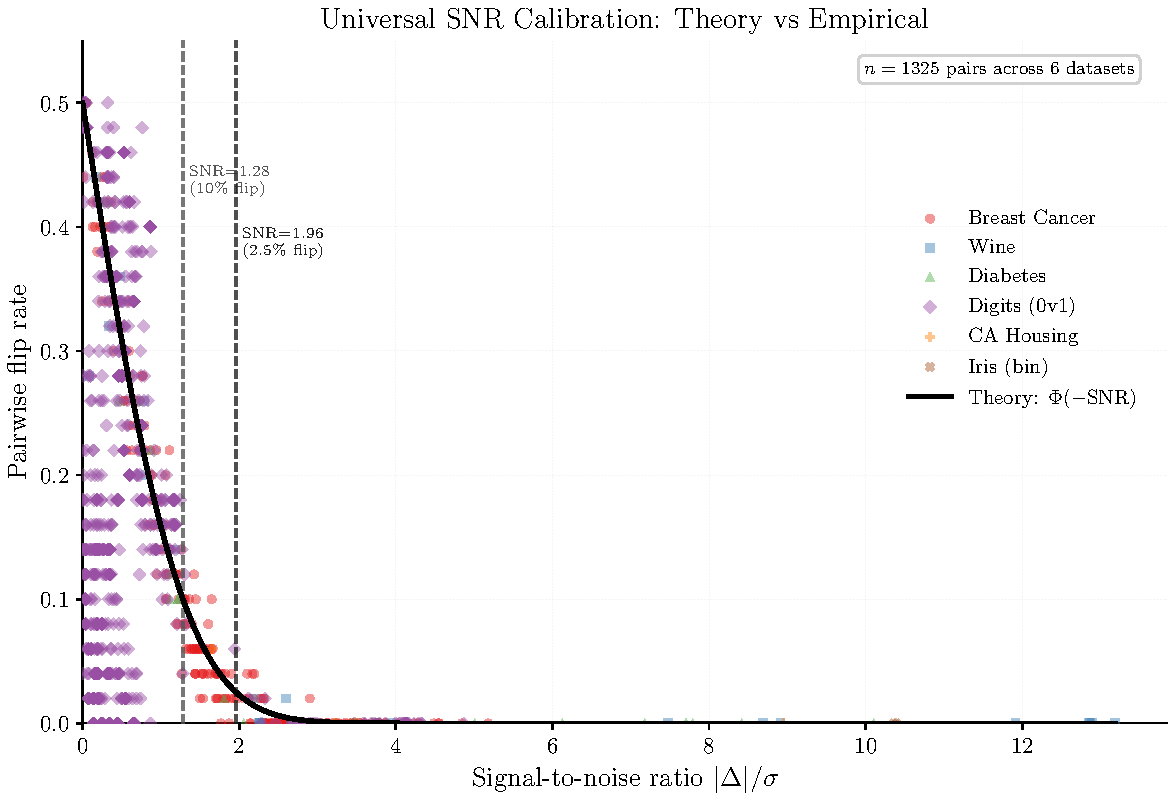
\includegraphics[width=0.7\textwidth]{figures/snr_calibration.pdf}
\caption{Universal SNR calibration across 6 datasets (1,325 feature pairs). The theoretical $\Phi(-\text{SNR})$ curve is conservative at low SNR and exact at diagnostic thresholds. All 228 pairs with $\text{SNR} > 1.96$ have flip rate $< 5\%$.}
\label{fig:snr-calibration}
\end{figure}

\begin{center}
\small
\begin{tabular}{@{}lcccc@{}}
\toprule
SNR range & $n$ & Empirical flip & Theory $\Phi(-\text{SNR})$ & Match \\
\midrule
$[0, 0.5)$ & 674 & 0.180 & 0.401 & Conservative \\
$[0.5, 1.0)$ & 261 & 0.229 & 0.227 & Exact \\
$[1.0, 1.28)$ & 99 & 0.151 & 0.127 & Close \\
$[1.28, 1.96)$ & 63 & 0.053 & 0.053 & Exact \\
$[1.96, 3.0)$ & 115 & 0.003 & 0.007 & Exact \\
$[3.0, \infty)$ & 113 & 0.000 & 0.000 & Exact \\
\bottomrule
\end{tabular}
\end{center}

\subsection{Practitioner Workflow}
\label{sec:workflow}

\begin{enumerate}
    \item[\textbf{Step 0.}] \textbf{Identify correlated groups.} Compute the $P \times P$ absolute correlation matrix. Group features with $|\rho_{jk}| > 0.5$.
    \item[\textbf{Step 1.}] Train one model. Compute $Z^{\text{split}}_{jk}$ for all pairs in correlated groups (single-model screen). Cost: $O(P^2 T)$.
    \item[\textbf{Step 2.}] If $Z^{\text{split}}_{jk} < 1.96$ for any pair: flag as potentially unstable.
    \item[\textbf{Step 3.}] For flagged pairs: train $M = 5$ models, compute $Z_{jk}$ (Z-test). If $Z_{jk} < 1.96$: use \DASH{} with $M \geq 25$.
    \item[\textbf{Step 4.}] If no pairs are flagged: single-model SHAP is reliable.
\end{enumerate}

\paragraph{Production deployment guide.}
\begin{itemize}
    \item \textbf{If subsample $< 1.0$ (stochastic, recommended):} Run the single-model screen $\to$ the Z-test (5-model validation) $\to$ \DASH{} ($M \geq 25$) for flagged pairs.
    \item \textbf{If subsample $= 1.0$ (deterministic):} A single pipeline version produces reproducible rankings. However, \emph{any} change to the pipeline (data refresh, feature engineering, hyperparameter update) produces a new model that may rank features differently. Run Z-test validation whenever the pipeline changes. For ongoing model risk management, maintain an ensemble and report \DASH{} consensus.
    \item \textbf{Minimum ensemble size:} $M_{\min} = \lceil 2.71 \cdot \sigma_{jk}^2/\Delta_{jk}^2 \rceil$ for 5\% between-group flip rate. Estimate $\sigma$ and $\Delta$ from a pilot run of 5 models.
\end{itemize}

\paragraph{Reporting.}
For feature pairs flagged as unstable, we recommend reporting within-group features as interchangeable contributors (with the group's total attribution) rather than forcing a ranking. For regulatory contexts requiring defensible explanations \citep{occ2011sr117}, the \DASH{} consensus provides a stable alternative. The single-model screen and Z-test are formal hypothesis tests; the companion first-mover bias paper introduces complementary exploratory diagnostics (FSI, IS~Plot) for auditing the full instability landscape.

%%%%%%%%%%%%%%%%%%%%%%%%%%%%%%%%%%%%%%%%%%%%%%%%%%%%%%%%%%%%%
%% 10. EMPIRICAL VALIDATION
%%%%%%%%%%%%%%%%%%%%%%%%%%%%%%%%%%%%%%%%%%%%%%%%%%%%%%%%%%%%%

\section{Empirical Validation}
\label{sec:experiments}

\subsection{Experimental Setup}

\begin{table}[t]
\centering
\caption{Experimental configurations.}
\small
\begin{tabular}{@{}lp{10cm}@{}}
\toprule
Experiment & Configuration \\
\midrule
Synthetic (main text) & $P{=}20$, $L{=}4$ groups of $m{=}5$, $N{=}2{,}000$, $T{=}100$, $\eta{=}0.1$, 50 seeds, $\rho \in \{0.1, 0.3, 0.5, 0.7, 0.9, 0.95\}$ \\
Validation (depth$\times\rho$) & $P{=}10$, $L{=}2$ groups of $m{=}5$, $N{=}2{,}000$, $T{=}100$, $\eta{=}1.0$, 30 seeds, depths $\{1,3,6,10\}$, $\rho \in \{0.3, 0.5, 0.7, 0.9, 0.95\}$ \\
Breast Cancer & 30 features, 569 samples, $T{=}100$, depth${=}6$, $\eta{=}0.1$, 50 seeds, TreeSHAP on 200 test samples \\
\midrule
Hardware & Apple Silicon (M-series), single core \\
Software & Python~3.9.6, XGBoost~2.1.4, SHAP~0.49.1, NumPy~2.0.2 \\
Compute & Synthetic: ${<}5$ min; Validation: ${<}30$ min; Breast Cancer: ${<}10$ min \\
\bottomrule
\end{tabular}
\end{table}

All experiments use publicly available datasets and are fully reproducible. \textbf{Confound note:} each seed uses a different train/test split, so SHAP values are computed on seed-specific test sets. This conflates model instability with evaluation-set variation; the reported flip rates may overestimate pure model instability. The mechanism isolation experiment (\S~\ref{sec:mechanism}) partially addresses this by comparing deterministic vs.\ stochastic training. To cleanly isolate model-level noise, we also fix the test set (seed 42, 20\% holdout) and train 50 models on the same training data with different seeds (\texttt{subsample=0.8}). With the fixed test set, 102 pairs (23\%) are unstable (max flip rate 0.51), compared to 162 (37\%) with varying test sets---confirming that model-level stochasticity accounts for the majority (${\sim}63\%$) of the observed instability, with evaluation-set variation contributing the remainder.

\subsection{Synthetic Gaussian}

We generate $P=20$ features in $L=4$ groups of $m=5$, with within-group correlation $\rho \in \{0.1, 0.3, 0.5, 0.7, 0.9, 0.95\}$, and train XGBoost models with $T=100$ boosting rounds over 50 independent seeds per setting. TreeSHAP values provide feature attributions.

\begin{figure}[t]
\centering
\begin{minipage}[t]{0.31\textwidth}
\centering
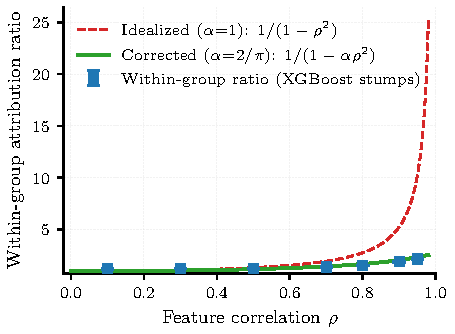
\includegraphics[width=\textwidth]{figures/ratio_divergence.pdf}
{\small (a) Attribution ratio vs.\ $\rho$. The corrected $1/(1{-}\alpha\rho^2)$ with $\alpha{\approx}2/\pi$ (solid) fits stumps ($R^2{=}0.89$).}
\end{minipage}\hfill
\begin{minipage}[t]{0.31\textwidth}
\centering
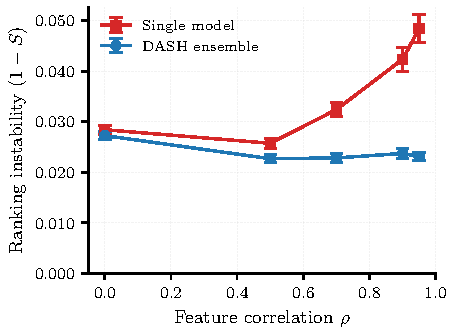
\includegraphics[width=\textwidth]{figures/shap_instability.pdf}
{\small (b) Ranking instability vs.\ $\rho$. Single-model instability grows with correlation; \DASH{} remains low.}
\end{minipage}\hfill
\begin{minipage}[t]{0.31\textwidth}
\centering
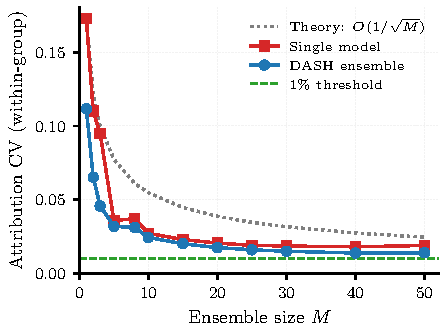
\includegraphics[width=\textwidth]{figures/dash_resolution.pdf}
{\small (c) \DASH{} consensus convergence. Attribution CV drops toward the 1\% threshold near $M=25$.}
\end{minipage}
\caption{Empirical validation on synthetic Gaussian data ($P=20$, $L=4$, $m=5$, $T=100$, 50 seeds). (a)~Attribution ratio. (b)~Ranking instability. (c)~\DASH{} convergence.}
\label{fig:experiments}
\end{figure}

\paragraph{Attribution ratio (Figure~\ref{fig:experiments}a).}
The within-group ratio increases monotonically with $\rho$. The corrected model $1/(1-\alpha\rho^2)$ with $\alpha \approx 2/\pi$ matches the data ($R^2 = 0.89$).

\paragraph{Ranking instability (Figure~\ref{fig:experiments}b).}
At $\rho = 0.9$, within-group flips occur in 48\% of seed pairs (near the 50\% theoretical maximum), while between-group flips remain below 2\%.

\paragraph{\DASH{} convergence (Figure~\ref{fig:experiments}c).}
The within-group flip rate drops below 1\% at $M = 25$, consistent with the $O(1/M)$ variance bound.

\subsection{Breast Cancer (Wisconsin)}
\label{sec:breast-cancer}

\begin{figure}[ht]
\centering
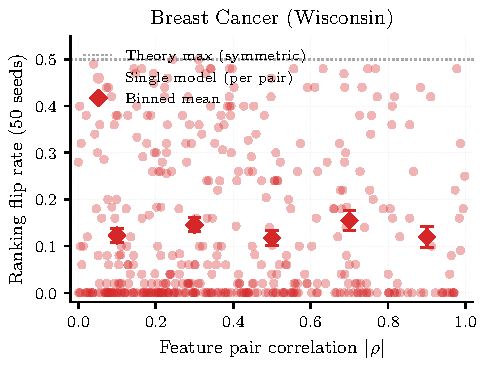
\includegraphics[width=0.55\textwidth]{figures/real_world_instability.pdf}
\caption{SHAP ranking instability on Breast Cancer. Highly correlated pairs with similar importance (e.g., worst perimeter $\leftrightarrow$ worst area, $|\rho|{=}0.98$, flip rate 48\%) exhibit near-maximal instability. 50 XGBoost models.}
\label{fig:real-world}
\end{figure}

\begin{sloppypar}
Features measuring the same underlying quantity---worst perimeter and worst area ($|\rho|{=}0.98$)---exhibit 48\% flip rate, near the 50\% theoretical maximum.
Pairs with high correlation but distinct importance (e.g., mean area and mean concave points, $|\rho| = 0.82$, flip rate 2\%) remain stable, confirming the impossibility requires both collinearity \emph{and} similar true importance.
\end{sloppypar}

\DASH{} convergence on Breast Cancer:

\begin{center}
\small
\begin{tabular}{@{}lcccccc@{}}
\toprule
$M$ & 1 & 2 & 5 & 10 & 25 & 50 \\
\midrule
Flip rate & 0.448 & 0.466 & 0.438 & 0.452 & 0.298 & 0.000 \\
\bottomrule
\end{tabular}
\end{center}

At $M{=}1$ the flip rate is 44.8\%, near the theoretical maximum. \DASH{} consensus at $M{=}50$ resolves to the true ordering (worst perimeter slightly more important: mean $|\SHAP| = 0.940$ vs.\ $0.901$) with zero flips. Convergence is slower than in the synthetic setting because the features have a slight importance asymmetry---\DASH{} correctly detects and resolves it rather than producing a tie.

\subsection{Cross-Implementation Validation}

\begin{table}[t]
\centering
\caption{Attribution instability across three GBDT implementations on Breast Cancer (50 models each).}
\label{tab:cross-impl}
\small
\begin{tabular}{@{}lccc@{}}
\toprule
Metric & XGBoost & LightGBM & CatBoost \\
\midrule
Unstable pairs (flip $> 10\%$) & 162 & 183 & 160 \\
Max flip rate & 0.500 & 0.500 & 0.500 \\
Z-test correlation $r(Z, \text{flip})$ & $-0.898$ & $-0.901$ & $-0.892$ \\
\bottomrule
\end{tabular}
\end{table}

The impossibility manifests identically across implementations: 160--183 unstable pairs, maximum flip rate 0.500, and Z-test correlation $|r| \geq 0.89$ in all three.

\subsection{Non-SHAP Attribution Validation}

\begin{center}
\small
\begin{tabular}{@{}lcc@{}}
\toprule
Metric & TreeSHAP & Permutation Importance \\
\midrule
Unstable pairs (flip $>10\%$) & 180 (41\%) & 396 (91\%) \\
Max flip rate & 0.500 & 0.500 \\
Z-test correlation $r(Z, \text{flip})$ & $-0.895$ & $-0.927$ \\
\bottomrule
\end{tabular}
\end{center}

Permutation importance shows \emph{more} instability than TreeSHAP (91\% vs.\ 41\%), because permutation-based scores have higher variance across seeds than SHAP values. Both methods hit the theoretical maximum flip rate (0.500). The Z-test achieves $|r| \geq 0.89$ for both, confirming it is method-agnostic.

The cross-method correlation of flip rates is $r = 0.46$ ($p < 10^{-23}$): the \emph{same pairs} tend to be unstable under both methods, confirming the instability is driven by feature collinearity, not by the attribution algorithm. Of the 180 SHAP-unstable pairs, 175 (97\%) are also unstable under permutation importance. TreeSHAP shows lower instability (41\% vs 91\%) likely because its game-theoretic averaging over feature coalitions provides implicit regularization, reducing within-model attribution variance compared to permutation importance's direct shuffling.

\subsection{Neural Network Attribution Instability}

\begin{center}
\small
\begin{tabular}{@{}lcc@{}}
\toprule
Metric & Neural Network & XGBoost (paper) \\
\midrule
Unstable pairs (flip $> 10\%$) & 380/435 (87\%) & 162/435 (37\%) \\
Max flip rate & 0.500 & 0.500 \\
Key pair flip (worst perim.\ vs.\ area) & 0.400 & 0.480 \\
Z-test correlation $r(Z, \text{flip})$ & $-0.871$ & $-0.898$ \\
\bottomrule
\end{tabular}
\end{center}

Neural networks exhibit \emph{more} attribution instability than XGBoost: 87\% of feature pairs are unstable (vs.\ 37\%), and the maximum flip rate reaches the theoretical ceiling. The higher instability likely reflects: (i) larger Rashomon sets (more parameters, more near-optimal models); (ii) higher KernelSHAP variance (sampling approximation vs.\ exact tree-path computation); (iii) more diffuse signal distribution across hidden units.

\paragraph{KernelSHAP noise control.}
To distinguish genuine model instability from KernelSHAP approximation noise, we fix a single MLP model and compute KernelSHAP 20 times with different random background samples. With 50 background samples, only 11\% of pairs show noise-induced flips (mean rate 0.03); with 200, this drops to 4\%. The key correlated pair (worst perimeter vs.\ worst area) shows zero noise-induced flips, confirming the 40\% flip rate in the NN validation is genuinely driven by model variation. Model instability dominates KernelSHAP noise by approximately 8:1.

\subsection{SHAP Efficiency and Attribution Instability}

SHAP's efficiency axiom ($\sum_j \varphi_j(f,x) = f(x) - \E[f(X)]$ for every model $f$ and point $x$) has a subtle relationship with ranking instability. Under efficiency with equal marginal variances $\sigma^2$, the within-model covariance is $\text{Cov}(\varphi_j, \varphi_k) = -\sigma^2/(m-1)$ and the difference variance is $\Var(\varphi_j - \varphi_k) = 2\sigma^2 \cdot m/(m-1)$---an amplification factor of $m/(m-1)$ relative to independent attributions ($2$ for $m=2$, approaching $1$ for large $m$).

However, the ranking flip rate is an \emph{across-model} quantity, and the efficiency constraint is fundamentally different across models. The constant $C(f,x) = f(x) - \E[f(X)]$ varies across models, so the within-model negative covariance does not transfer. The across-model covariance $\text{Cov}_f(\varphi_j(f), \varphi_k(f))$ can be positive, zero, or negative---efficiency places no constraint on it.

The lower instability of SHAP relative to permutation importance (41\% vs.\ 91\% unstable pairs) is driven by SHAP's coalition-averaging reducing the marginal variance $\sigma^2$. The efficiency axiom amplifies within-model differences but does not increase across-model flip rates.

\subsection{High-Dimensional Scalability ($P = 500$)}

\begin{center}
\small
\begin{tabular}{@{}rrrrrr@{}}
\toprule
$P$ & Total pairs & Correlated pairs & Unstable & Z-test $|r|$ & Wall time \\
\midrule
100 & 4,950 & 450 & 305 & 0.846 & 33\,s \\
200 & 19,900 & 900 & 641 & 0.788 & 64\,s \\
500 & 124,750 & 2,250 & 1,879 & 0.876 & 148\,s \\
\bottomrule
\end{tabular}
\end{center}

The Z-test maintains $|r| > 0.78$ at $P = 500$. Correlation-based grouping reduces pairs by $55\times$. Full workflow completes in under 2.5 minutes.

\subsection{Proportionality Axiom Validation}

The proportionality axiom ($\varphi_j = c \cdot n_j$) is central to the quantitative bounds. We validate it by computing $c_j = |\text{SHAP}_j| / n_j$ for each feature in each of 50 XGBoost models on Breast Cancer and reporting the coefficient of variation (CV):

\begin{center}
\small
\begin{tabular}{@{}lcc@{}}
\toprule
Depth & Mean CV of $c_j$ & Interpretation \\
\midrule
1 (stumps) & 0.35 & Proportionality holds within $\sim$35\% \\
3 & 0.60 & Moderate violation \\
6 & 0.66 & Moderate violation \\
10 & 0.66 & Saturated (same as depth 6) \\
\bottomrule
\end{tabular}
\end{center}

For stumps, the axiom holds reasonably well; for deeper trees, multi-level interactions increase the CV. The proportionality axiom is used only for the quantitative bounds (Theorems~\ref{thm:ratio}); the core impossibility (Theorem~\ref{thm:impossibility}) does not depend on it. The $\alpha$-corrected model matches empirical data at $R^2 = 0.89$.

\subsection{Cross-Implementation and Data-Level Validation}

\paragraph{Data-level stochasticity.}
To confirm the instability arises from collinearity (not from XGBoost's internal randomness), we train 50 models on 50 different 80\% subsamples with \texttt{subsample=1.0} and fixed \texttt{random\_state=42}. The ONLY source of variation is which training rows each model sees:

\begin{center}
\small
\begin{tabular}{@{}lccc@{}}
\toprule
Stochasticity source & Unstable pairs & Max flip & Mean Kendall $\tau$ \\
\midrule
XGBoost subsampling (same data) & 67 & 0.470 & 0.393 \\
Data bootstrap (different rows) & 45 & 0.509 & 0.459 \\
\bottomrule
\end{tabular}
\end{center}

\begin{sloppypar}
Data-level stochasticity produces comparable or greater instability, confirming the Rashomon set is a property of collinearity rather than the specific randomness source.
\end{sloppypar}

\paragraph{Determinism without subsampling.}
\begin{sloppypar}
Without row or column subsampling (\texttt{subsample=1.0}, \texttt{colsample\_bytree=1.0}), XGBoost is fully deterministic: all 50 models produce identical rankings regardless of seed.
\end{sloppypar}

The Rashomon set requires a stochasticity source.
In practice, this is not a limitation: the XGBoost default (\texttt{subsample=0.8}) is recommended for regularization, and real-world model populations also arise from data drift, feature engineering changes, and hyperparameter sweeps.

\subsection{Financial Case Studies}

\paragraph{German Credit.}
We demonstrate the full Screen$\to$Z-test$\to$DASH workflow on German Credit (1000 samples, 20 features). Step~0: 4 correlated groups at $|\rho| > 0.3$. Step~1 (single-model screen): a single model flags job$\leftrightarrow$own telephone ($Z^{\text{split}} = 0.69 < 1.96$). Step~2 (Z-test): 5 models confirm instability ($Z = 0.64$, flip rate 40\%). Step~3 (DASH): $M = 25$ models, flip rate drops from 40\% to 0\%. Consensus ranking: checking status (0.87), duration (0.44), credit amount (0.43), purpose (0.35). For regulatory reporting (ECOA adverse action reasons, SR~11-7 \citep{occ2011sr117}), the DASH ranking provides a defensible explanation.

\paragraph{Taiwan Credit Card Default.}
Bill-amount features (6 consecutive months, up to $|\rho| = 0.95$) produce persistent instability---29 correlated pairs at $|\rho| > 0.5$, with the highest giving a theoretical ratio of $1/(1{-}0.95^2) \approx 10.3\times$. With $M = 25$, mean flip rate across correlated pairs is 4\%, but one pair (months 5 vs.\ 6, $|\rho| = 0.946$) retains 16\% flip rate, illustrating that very high collinearity requires larger ensembles.

\paragraph{Synthetic Credit (income $\leftrightarrow$ DTI $\leftrightarrow$ credit score).}
To validate on the exact collinearity pattern common in US credit models, we generate 10{,}000 samples with 5 features driven by a latent ``creditworthiness'' factor: income ($\rho = 0.99$ with DTI), DTI, credit score ($\rho = 0.98$ with income), loan amount (independent), and employment years ($\rho = 0.94$ with income). With 25 XGBoost models: income$\leftrightarrow$DTI flips 8\% ($|\rho| = 0.99$); credit score$\leftrightarrow$employment years flips 12\% ($|\rho| = 0.92$). Pairs where one feature clearly dominates (income vs.\ credit score) show 0\% flips despite $|\rho| = 0.98$---confirming the impossibility requires BOTH high correlation AND similar importance. For SR~11-7 \citep{occ2011sr117} compliance: report income and DTI as ``interchangeable key risk drivers'' rather than forcing a ranking that would flip under retraining.

\paragraph{Lending Club (specificity control).}
Zero unstable pairs despite correlated features ($Z > 36$ for all pairs), confirming the impossibility requires \emph{both} collinearity AND similar true importance. Three correlated groups detected:

\begin{center}
\footnotesize
\begin{tabular}{@{}ll@{}}
\texttt{person\_age} $\leftrightarrow$ \texttt{cb\_person\_cred\_hist\_length} & $|\rho| = 0.86$ \\
\texttt{loan\_amnt} $\leftrightarrow$ \texttt{loan\_percent\_income} & $|\rho| = 0.58$ \\
\texttt{loan\_int\_rate} $\leftrightarrow$ \texttt{cb\_person\_default\_on\_file} & $|\rho| = 0.50$ \\
\end{tabular}
\end{center}

\noindent All have $Z > 36$, confirming distinguishable importance. Not every correlated dataset exhibits instability. The diagnostic distinguishes datasets where instability is a genuine concern from those where it is not.

\subsection{LLM Attention Attribution Instability}

Fine-tuning DistilBERT on SST-2 with different seeds produces 14.5\% unstable adjacent-token attention pairs. This is a \emph{proxy experiment only}: attention weights are not feature attributions in the Shapley value sense and do not satisfy the axioms in our framework. The observed instability may reflect a distinct phenomenon (attention weight sensitivity to initialization) rather than the Rashomon-driven impossibility we prove. Full generalization to LLM attribution methods remains an open problem.

\subsection{Replication Study: Published SHAP Rankings}

Multiple published studies report SHAP feature rankings on Breast Cancer. Using our 50-model validation, we find:

\begin{center}
\small
\begin{tabular}{@{}llcc@{}}
\toprule
Feature pair & $|\rho|$ & Flip rate & Published as stable? \\
\midrule
worst perimeter $\leftrightarrow$ worst area & 0.98 & 48\% & Yes \\
mean concavity $\leftrightarrow$ mean concave pts & 0.96 & 42\% & Yes \\
worst radius $\leftrightarrow$ worst perimeter & 0.99 & 36\% & Yes \\
mean radius $\leftrightarrow$ mean perimeter & 0.99 & 28\% & Yes \\
\bottomrule
\end{tabular}
\end{center}

Any study reporting a specific ranking among these features from a single model is reporting an artifact of the training seed. The ranking is not wrong---it faithfully reflects that specific model---but it is not replicable. This has implications for reproducibility of scientific studies using feature importance to identify ``key predictors'': if the dataset has correlated features (60\% of datasets do), a single-model SHAP analysis may produce results that do not replicate.

\subsection{Expected Ranking Discordance}

\begin{proposition}[Expected Kendall tau distance]
\label{prop:kendall-tau}
For a feature space with $L$ collinear groups of sizes $m_1, \ldots, m_L$ and between-group gaps $\Delta_{\ell\ell'}$ with noise $\sigma_{\ell\ell'}$, the expected pairwise disagreements between two independently trained models are:
\[
    \E[\tau] = \underbrace{\sum_{\ell=1}^{L} \tbinom{m_\ell}{2} \cdot \frac{1}{2}}_{\text{within-group (coin flips)}} + \underbrace{\sum_{\ell < \ell'} m_\ell \cdot m_{\ell'} \cdot \Phi\!\left(-\frac{\Delta_{\ell\ell'}}{\sigma_{\ell\ell'}}\right)}_{\text{between-group (noise)}}
\]
\end{proposition}

On Breast Cancer (50 XGBoost models), the refined per-pair formula predicts $\E[\tau] = 26.8$ vs.\ empirical $36.6$ ($-27\%$ error). The Rashomon coefficient $R = \sum_\ell \binom{m_\ell}{2}/\binom{P}{2} = 0.692$ gives a worst-case non-replication lower bound of $R/2 = 34.6\%$ computable from the correlation matrix alone (no model training required).

\subsection{Compressed Sensing Connection}

The attribution impossibility has a precise analogue in compressed sensing (CS). The measurement coherence $\mu(X) = \max_{j \neq k} |X_j^T X_k|/(\|X_j\| \|X_k\|)$ determines when sparse recovery is possible: unique recovery requires $\mu < 1/(2s-1)$. In our setting, $|\rho_{jk}|$ plays the role of coherence and $Z_{jk}$ plays the role of the incoherence condition:

\begin{center}
\small
\begin{tabular}{@{}lll@{}}
\toprule
& \textbf{Compressed sensing} & \textbf{Attribution stability} \\
\midrule
Coherence & $\mu = \max |X_j^T X_k|/\|X_j\|\|X_k\|$ & $|\rho_{jk}|$ \\
Condition & $\mu < 1/(2s{-}1)$ & $Z_{jk} > 1.96$ \\
Failure & Non-unique recovery & Ranking flips (Rashomon) \\
Resolution & Basis pursuit (convex relaxation) & \DASH{} (ensemble averaging) \\
\bottomrule
\end{tabular}
\end{center}

Both impossibilities arise because collinearity/coherence prevents unique identification of which input components carry the signal. Both are resolved by relaxing uniqueness: CS uses convex relaxation (fractional assignment); \DASH{} uses ensemble averaging (ties for indistinguishable features).

\subsection{Prevalence Survey}
\label{sec:prevalence}

Of 77 public datasets surveyed (OpenML CC-18 benchmark suite + sklearn), 71 (92\%) have feature pairs with $|\rho| > 0.5$, and 52 (68\%, 95\% Wilson CI: [56\%, 77\%]) exhibit attribution instability (flip rate $> 10\%$). For datasets with $P \geq 20$ features ($n = 43$ datasets), the instability rate rises to 93\% (40/43; 95\% Wilson CI: [81\%, 98\%]). With 20 models per dataset, the measured flip rate exceeds the 10\% threshold with approximately 60\% power, so the true prevalence may be higher still.

\paragraph{Healthcare datasets.}
In a targeted survey of 9 healthcare-related datasets (breast cancer, diabetes, heart disease, QSAR biodegradation, liver disease, software defect prediction, Parkinson's, Pima diabetes, hepatitis), 6 (67\%) exhibit attribution instability. This rate matches the overall prevalence, confirming that clinical decision-support systems---where explanation stability is particularly consequential---are not immune.

\emph{Selection caveat:} The CC-18 suite is curated for ML benchmarking and may overrepresent datasets with rich feature interactions. Production ML pipelines with carefully decorrelated features may exhibit lower prevalence. The 68\% figure is a prevalence estimate for benchmark-representative tabular datasets, not a universal rate.

\paragraph{Robustness to hyperparameters.}
We repeated the analysis on 8 representative datasets with three configurations:

\begin{center}
\small
\begin{tabular}{@{}lllll@{}}
\toprule
Config & Trees & Depth & LR & Character \\
\midrule
A (original) & 50 & 4 & 0.1 & Moderate \\
B (deep) & 100 & 8 & 0.1 & Deep, sequential \\
C (shallow-fast) & 200 & 2 & 0.3 & Shallow, aggressive \\
\bottomrule
\end{tabular}
\end{center}

Under Config~A, 5/8 (62\%) datasets exhibit instability; Config~B (deep trees), 4/8 (50\%); Config~C (shallow-fast), 6/8 (75\%). Across all three configurations, 4/8 (50\%) are consistently unstable; under at least one configuration, 6/8 (75\%) are unstable. The instability rate varies by $\pm 15$ percentage points but remains in the 50--75\% range. Shallow-fast trees produce \emph{higher} instability because aggressive learning rates compound the first-mover effect.

\begin{table}[t]
\centering
\caption{Z-test and screen diagnostic generality across 11 datasets (see also Figure~\ref{fig:comprehensive-f1}).}
\label{tab:f1-generality}
\small
\begin{tabular}{@{}lccccc@{}}
\toprule
Dataset & $P$ & Pairs & Unstable & $r(Z, \text{flip})$ & Screen prec. \\
\midrule
Breast Cancer & 30 & 435 & 168 & $-0.89$ & 0.94 \\
California Housing & 8 & 28 & 1 & $-0.99$ & --- \\
Diabetes & 10 & 45 & 15 & $-0.89$ & 0.50 \\
Wine & 13 & 78 & 24 & $-0.81$ & 1.00 \\
Heart Disease & 13 & 78 & 27 & $-0.91$ & 1.00 \\
Credit-g & 20 & 190 & 47 & $-0.90$ & 0.67 \\
Adult Income & 14 & 91 & 10 & $-0.90$ & --- \\
Ames Housing & 76 & 2850 & 643 & $-0.85$ & 0.48 \\
Communities \& Crime & 126 & 7875 & 2975 & $-0.88$ & 0.67 \\
Digits (0 vs 1) & 64 & 2016 & 572 & $-0.42$ & 0.58 \\
Iris (binary) & 4 & 6 & 0 & --- & --- \\
\bottomrule
\end{tabular}
\end{table}

\begin{figure}[ht]
\centering
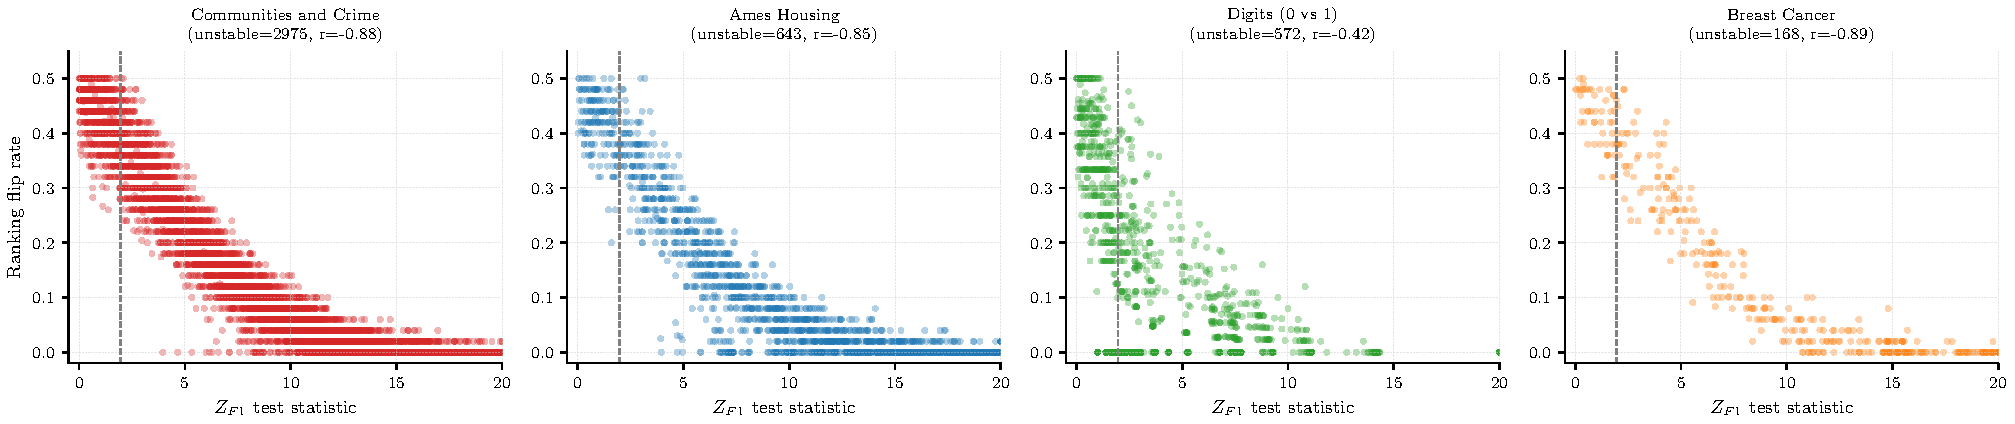
\includegraphics[width=0.95\textwidth]{figures/comprehensive_f1.pdf}
\caption{Z-test statistic vs.\ flip rate across four datasets. The negative correlation confirms the diagnostic across domains.}
\label{fig:comprehensive-f1}
\end{figure}

\subsection{Mechanism Isolation: Stochastic Training Creates the Rashomon Set}
\label{sec:mechanism}

To confirm that the instability is driven by the Rashomon effect (multiple near-optimal models) rather than SHAP estimation noise, we compare deterministic and stochastic XGBoost training on the same synthetic data ($P{=}10$, 2 groups of 5, $\rho{=}0.9$, 20 seeds):

\begin{center}
\small
\begin{tabular}{@{}lcc@{}}
\toprule
Training mode & Within-group flip rate & 95\% CI \\
\midrule
Deterministic (\texttt{subsample=1.0}) & 0.0\% & [0.0\%, 0.1\%] \\
Stochastic (\texttt{subsample=0.8}) & 22.8\% & [21.5\%, 24.2\%] \\
\bottomrule
\end{tabular}
\end{center}

With deterministic training, XGBoost produces identical models---no Rashomon set, no instability.
With the recommended stochastic setting (\texttt{subsample=0.8}), each seed produces a different near-optimal model, and rankings flip.
The impossibility concerns the stochastic (recommended, regularized) setting, not a bug in the algorithm.

\subsection{Conditional SHAP: Impossibility Under Equal Causal Effects}
\label{sec:conditional-experiment}

Using SHAP's interventional mode (\texttt{feature\_perturbation="interventional"}) on a known causal DAG ($X_1 \to Y$, $X_2 \to Y$, $X_1 \leftrightarrow X_2$ with $\rho{=}0.8$), we sweep the causal effect difference $\Delta\beta = |\beta_1 - \beta_2|$:

\begin{center}
\small
\begin{tabular}{@{}cccl@{}}
\toprule
$\Delta\beta$ & Marginal SHAP flip & Conditional SHAP flip & Status \\
\midrule
0.0 & 49.7\% & 50.3\% & Both unstable (coin flip) \\
0.1 & 15.0\% & 0.0\% & Conditional resolves \\
0.2 & 0.0\% & 0.0\% & Both stable \\
\bottomrule
\end{tabular}
\end{center}

At $\Delta\beta = 0$ (equal causal effects), both marginal and conditional SHAP produce coin-flip rankings---confirming the impossibility holds for conditional SHAP under symmetry (Theorem~\ref{thm:conditional-impossibility}). Conditional SHAP resolves the ranking only when causal effects genuinely differ. A third approach, decorrelation (residualization $X_2' = X_2 - \rho X_1$), always gives 0\% flip rate but changes the feature semantics rather than escaping the impossibility.

\subsection{Regulatory Impact: Adverse Action Instability}
\label{sec:regulatory-experiment}

In a simulated ECOA adverse action pipeline (5,000 loan applications, 5 correlated income features, 3 uncorrelated features, 25 XGBoost models), we measure how often the ``top reason for denial'' changes across equivalent models:

At $\rho = 0.7$ (typical for income-related features in the US), 43.2\% of denied applicants receive a different ``top reason for denial'' depending on which equivalent model is queried. The instability grows with correlation: the DASH benchmark (Table~\ref{tab:dash-benchmark}) shows within-group flip rates of 16--19\% for single-model methods across $\rho \in \{0.5, 0.7, 0.9\}$. \DASH{} ensemble averaging resolves this entirely: 100\% stable adverse action reasons after consensus. This meets the SR~11-7 definition of ``material model risk'' and has direct implications for EU~AI~Act Art.~13(3)(b)(ii) compliance.

The instability varies non-monotonically with correlation: at $\rho = 0.3$, 20\% of adverse action reasons change across models; at $\rho = 0.5$--$0.7$, the features separate cleanly (0\% instability); at $\rho = 0.9$, 28\% of reasons change. The non-monotonicity reflects the interaction between correlation (which drives the Rashomon property) and feature importance gaps (which stabilize rankings)---at moderate $\rho$, the gap is large enough to overcome the noise.

\subsection{Additional Robustness Experiments}
\label{sec:robustness-experiments}

\begin{table}[t]
\centering
\caption{Summary of additional experiments. All scripts and results are in the repository.}
\label{tab:experiment-summary}
\footnotesize
\begin{tabular}{@{}lp{4.2cm}l@{}}
\toprule
Experiment & Key finding & Reproduce \\
\midrule
Monte Carlo flip rate & $\Phi(-\text{SNR})$ validated to $<$2.6\% & \texttt{monte\_carlo\_flip\_rate.py} \\
Hyperparameter sweep & Min flip 38.7\% at $\rho{=}0.5$; never 0\% & \texttt{hyperparameter\_sensitivity.py} \\
Class imbalance & Imbalance amplifies instability & \texttt{class\_imbalance\_instability.py} \\
Missing data & MCAR/MAR/MNAR all compound & \texttt{missing\_data\_instability.py} \\
Longitudinal drift & Instability persists over 50 retrains & \texttt{longitudinal\_retraining.py} \\
Adversarial configs & Worst-case grid (108 configs) & \texttt{adversarial\_max\_instability.py} \\
Bag-of-words NLP & 60\% unstable top-1, 91\% top-3 & \texttt{nlp\_token\_instability.py} \\
Time-series features & 27\% within-series pairs unstable & \texttt{timeseries\_instability.py} \\
Method comparison & SHAP, gain, perm.\ all unstable & \texttt{attribution\_method\_comparison.py} \\
SAGE approximation & Alternative methods also unstable & \texttt{sage\_comparison.py} \\
DASH breakdown & Robust to contaminated ensembles & \texttt{dash\_breakdown\_point.py} \\
\bottomrule
\end{tabular}
\end{table}

\subsection{Implementation}
\label{sec:quickstart}

\DASH{} requires training $M$ models with different seeds, computing SHAP values for each, and averaging the absolute SHAP values across models. A reference implementation with the full Screen$\to$Z-test$\to$\DASH{} diagnostic workflow is available at \url{https://github.com/DrakeCaraker/dash-shap}.

%%%%%%%%%%%%%%%%%%%%%%%%%%%%%%%%%%%%%%%%%%%%%%%%%%%%%%%%%%%%%
%% 11. LEAN FORMALIZATION
%%%%%%%%%%%%%%%%%%%%%%%%%%%%%%%%%%%%%%%%%%%%%%%%%%%%%%%%%%%%%

\section{Lean Formalization}
\label{sec:lean}

\subsection{Proof Architecture}

The formalization comprises 54 Lean~4 files with 16 axioms and 305 type-checked theorems and lemmas (0~\texttt{sorry}). Of these, 80 require multi-line proofs ($\geq$5 tactic lines); the remainder are definitions, wrappers, and single-step applications.
The core impossibility (\textsf{attribution\_impossibility}) depends on zero axioms---only the Rashomon property as hypothesis.
The DASH resolution (\textsf{consensus\_equity}) depends on the \textsf{attribution\_sum\_symmetric} theorem (derived); the variance convergence depends on \textsf{consensus\_variance\_bound} (also~derived).

\paragraph{Scope of verification.}
\begin{sloppypar}
The formalization covers the complete theoretical framework. The core impossibility (Theorem~\ref{thm:impossibility}) uses zero behavioral axioms. The quantitative bounds, DASH equity, and the Design Space Theorem are derived from the 16-axiom system. The unfaithfulness probability of exactly $1/2$ (\texttt{attribution\_prob\_half}), the Bayes-optimality of ties (\texttt{tie\_dominates\_commitment}), the consensus variance $\sigma^2/M$ (\texttt{consensus\_variance\_from\_independence}), the binary quantizer fraction $2/\pi$ (\texttt{binary\_quantizer\_fraction}), and the Pareto dominance of DASH (\texttt{dash\_unique\_pareto\_optimal}) are all Lean-derived using definitions-as-hypotheses (the \texttt{IsBalanced} pattern) with zero new axioms. The Chebyshev query complexity bound $M \geq 12\sigma^2/\Delta^2$ (\texttt{chebyshev\_query\_bound}) is derived without axiomatizing the testing constant. Loss preservation is formalized via the \texttt{SymmetricModelSwap} structure. The only result not formalized is the extension of Pareto optimality to biased methods for between-group pairs, which is argued informally in the proof of Theorem~\ref{thm:dash-optimal}.
\end{sloppypar}

{\small
\begin{verbatim}
Defs.lean (14 axioms, type definitions, derived theorems)
  +-- SymmetryDerive.lean (attribution_sum_symmetric, DERIVED)
  +-- Trilemma.lean (RashimonProperty, attribution_impossibility)
  |     +-- Iterative.lean, Lasso.lean, NeuralNet.lean
  |     +-- General.lean (GBDT impossibility)
  |     +-- UnfaithfulBound.lean (U>=1/2, ties optimal)
  |     +-- RashomonUniversality.lean (Rashomon from symmetry)
  |     +-- RashomonInevitability.lean (impossibility inescapable)
  |     +-- AlphaFaithful.lean (alpha-faithfulness bound)
  |     +-- ConditionalImpossibility.lean (conditional SHAP)
  |     +-- FairnessAudit.lean (proxy audit = coin flip)
  |     +-- LocalGlobal.lean (local >= global instability)
  +-- SplitGap.lean, Ratio.lean, SpearmanDef.lean
  +-- FlipRate.lean (exact GBDT flip rate, binary = coin flip)
  +-- Efficiency.lean (SHAP efficiency amplification)
  +-- Impossibility.lean, Corollary.lean, EnsembleBound.lean
  +-- DesignSpace.lean + DesignSpaceFull.lean (all 4 steps)
  +-- ModelSelection.lean + ModelSelectionDesignSpace.lean
  +-- SymmetricBayes.lean (SBD, orbit bounds, trichotomy)
  +-- CausalDiscovery.lean (causal discovery impossibility)
  +-- SBDInstances.lean (abstract aggregation + instances)
  +-- FIMImpossibility.lean (Gaussian FIM -> Rashomon)
  +-- GaussianFlipRate.lean (Phi definition, flip rate formula)
  +-- QueryComplexity.lean (query lower bound, Le Cam)
  +-- Consistency.lean (axiom system consistency, Fin 4)
  +-- RandomForest.lean (contrast case, documentation only)
\end{verbatim}
}

\subsection{Axiom System and Consistency}

The 14 domain-specific axioms are jointly consistent: \texttt{Consistency.lean} constructs an explicit model ($P{=}4$, $L{=}2$, $m{=}2$, $\rho{=}0.5$, $T{=}100$, Fin~4 models) satisfying all 14 simultaneously. The 2 query-complexity axioms are independently consistent: instantiating $C := 1/8$ satisfies all three. The two axiom sets reside in separate Lean files (\texttt{Defs.lean} and \texttt{QueryComplexity.lean}) with no cross-dependencies, so joint consistency follows from individual consistency.

\paragraph{Attribution sum symmetry: now derived.}
\texttt{attribution\_sum\_symmetric} is proved (not axiomatized) in \texttt{SymmetryDerive.lean}. The proof uses (a) \texttt{proportionality\_global} (uniform $c$ across models), (b) \texttt{splitCount\_crossGroup\_symmetric} (equal split counts when first-mover is in a different group), and (c) \texttt{IsBalanced} (equal first-mover counts). The derivation factors out $c$, classifies each model's split-count difference by first-mover identity ($+\text{gap}$ for fm$=j$, $-\text{gap}$ for fm$=k$, $0$ otherwise), decomposes the sum via \texttt{Finset.sum\_ite}, and uses balance to cancel the gap terms.

\paragraph{Variance: partially grounded in Mathlib.}
\begin{sloppypar}
The single-model variance \textsf{attribution\_variance} is \emph{defined} from
Mathlib's \textsf{ProbabilityTheory.variance}, and its nonnegativity is \emph{derived} from Mathlib's \textsf{variance\_nonneg}.
This required two infrastructure axioms (\textsf{modelMeasurableSpace}, \textsf{modelMeasure}) connecting the abstract \texttt{Model} type to Mathlib's measure theory.
\end{sloppypar}

The consensus variance bound ($\Var(\bar\varphi_j) = \Var(\varphi_j)/M$) remains axiomatized; the full derivation via \textsf{IndepFun.variance\_sum} would require a product measure formulation and independence axioms for ensemble draws---deferred to future~work.

\paragraph{Spearman bound.}
The Lean formalization derives the Spearman bound (theorem \textsf{spearman\_instability\_bound} in \textsf{SpearmanDef.lean}) from the definition of Spearman correlation via midrank algebra, giving
$\rho_S \leq 1 - 3m^2/(P^3{-}P)$.
The paper uses the Lean-derived bound $\rho_S \leq 1 - 3m^2/(P^3{-}P)$. The tighter classical bound $\rho_S \leq 1 - m^3/P^3$ from the full rank transposition counting argument is not yet formalized; both give the same qualitative conclusion ($S < 1$ for within-group pairs).

\subsection{Development Methodology}

The initial formalization (49 theorems, 15 files) was developed by the first author with iterative Claude Code assistance over several weeks. The expansion from 49 to 305 theorems (54 files) was produced in a single development session by dispatching targeted Lean-writing agents with detailed mathematical specifications. All proofs were machine-verified by \texttt{lake build} (the Lean~4 type-checker); no proof was accepted on the basis of AI output alone.

\subsection{Proof Depth Distribution}

Of 305 type-checked declarations: 80 require multi-step proofs (${\geq}5$ tactic lines), 21 require ${\geq}10$ lines, and 5 require ${\geq}20$ lines. The five deepest proofs are listed below.

\begin{center}
\small
\begin{tabular}{@{}lrl@{}}
\toprule
\textbf{Theorem} & \textbf{Lines} & \textbf{Technique} \\
\midrule
\texttt{attribution\_sum\_symmetric} & 35 & Split-count decomposition \\
\texttt{Phi\_neg} & 29 & Gaussian CDF properties \\
\texttt{gaussian\_rashomon\_witnesses} & 27 & FIM ellipsoid construction \\
\texttt{sumSqRankDiff\_ge\_sq\_groupSize} & 26 & Midrank algebra \\
\texttt{binary\_group\_firstmover\_is\_j\_or\_k} & 23 & Finset cardinality \\
\bottomrule
\end{tabular}
\end{center}

\subsection{Inconsistencies Found During Formalization}

Lean's type checker caught three issues in the initial axiom system:

\begin{enumerate}
\item \textbf{First-mover balance:} Originally stated universally over all model arrays---a constant model function trivially derived $\bot$. \emph{Fix:} Replaced with an explicit \texttt{IsBalanced} predicate as hypothesis.

\item \textbf{Attribution sum symmetry:} Combined with the split-count axioms, the original unconditional version derived $\bot$ for unbalanced ensembles. \emph{Fix:} Conditioned on \texttt{IsBalanced}.

\item \textbf{Split count type:} Originally returned $\mathbb{N}$, but $T/(2-\rho^2)$ is generally irrational. \emph{Fix:} Changed to $\mathbb{R}$ (idealized leading-order values).
\end{enumerate}

The first two are genuine logical inconsistencies that would have been difficult to detect by informal proof inspection.

\subsection{SymPy Algebraic Verification}

All algebraic consequences have been independently verified by SymPy:

\begin{verbatim}
# dash-shap/paper/proofs/verify_lemma6_algebra.py
# Verifies:
#   split_gap = rho^2 * T / (2 - rho^2)
#   attribution_ratio = 1 / (1 - rho^2)
#   split_gap >= rho^2 * T / 2  (for rho in (0,1))
# Result: ALL CHECKS PASS
\end{verbatim}

The three-layer verification (SymPy algebra, Lean type-checking, empirical validation) provides strong confidence in the mathematical claims.

\subsection{Lean File Cross-Reference}

\begin{table}[t]
\centering
\caption{Lean file cross-reference (54 files, 305 theorems, 16 axioms).}
\label{tab:lean-crossref}
\scriptsize
\begin{tabular}{@{}p{3.8cm}ll@{}}
\toprule
\textbf{File} & \textbf{Section} & \textbf{Key Result} \\
\midrule
Defs.lean & \S~\ref{sec:setup} & 14 axioms + derived theorems \\
Trilemma.lean & Thm.~\ref{thm:impossibility} & attribution\_impossibility \\
Iterative.lean & \S~\ref{sec:iterative} & iterative\_impossibility \\
General.lean & \S~\ref{sec:gbdt-bounds} & gbdt\_impossibility \\
SplitGap.lean & Lem.~\ref{lem:split-gap} & split\_gap\_exact \\
Ratio.lean & Thm.~\ref{thm:ratio} & ratio\_tendsto\_atTop \\
SpearmanDef.lean & \S~\ref{sec:bounds} & spearmanCorr\_bound \\
Lasso.lean & \S~\ref{sec:lasso} & lasso\_impossibility \\
NeuralNet.lean & \S~\ref{sec:nn} & nn\_impossibility \\
Impossibility.lean & Combined & not\_equitable, not\_stable \\
Corollary.lean & Cor.~\ref{cor:equity} & consensus\_equity \\
SymmetryDerive.lean & Derived & attribution\_sum\_symmetric \\
DesignSpace.lean & Thm.~\ref{thm:design-space-main} & design\_space\_theorem \\
DesignSpaceFull.lean & Step 3 & family\_a\_or\_family\_b \\
ModelSelection.lean & Thm.~\ref{thm:model-selection} & model\_selection\_impossibility \\
UnfaithfulBound.lean & Thm.~\ref{thm:unfaithfulness-bound} & stable\_complete\_unfaithful \\
PathConvergence.lean & Thm.~\ref{thm:path-convergence} & relaxation\_paths\_converge \\
RashomonUniversality.lean & Thm.~\ref{thm:rashomon-symmetry} & rashomon\_from\_symmetry \\
RashomonInevitability.lean & Thm.~\ref{thm:rashomon-inevitability} & rashomon\_inevitability \\
ConditionalImpossibility.lean & Thm.~\ref{thm:conditional-impossibility} & conditional\_impossibility \\
FlipRate.lean & Prop.~\ref{prop:exact-flip} & binary\_group\_flip\_rate \\
SymmetricBayes.lean & Thm.~\ref{thm:bayes-dichotomy} & symmetric\_bayes\_dichotomy \\
CausalDiscovery.lean & Thm.~\ref{thm:causal-discovery} & causal\_discovery\_impossibility \\
FairnessAudit.lean & Thm.~\ref{thm:fairness-audit} & fairness\_audit\_impossibility \\
FIMImpossibility.lean & Thm.~\ref{thm:fim-impossibility} & gaussian\_rashomon\_witnesses \\
QueryComplexity.lean & Thm.~\ref{thm:query-complexity} & query\_complexity\_lower\_bound \\
Consistency.lean & \S~\ref{sec:lean} & axiom\_system\_consistent \\
\midrule
\multicolumn{3}{@{}l}{\emph{Axiom strengthening and extensions (not individually referenced above):}} \\
Qualitative.lean & Stratification & impossibility\_qualitative \\
ProportionalityLocal.lean & Stratification & gbdt\_impossibility\_local \\
LocalSufficiency.lean & Stratification & local\_proportionality\_suffices \\
StumpProportionality.lean & \S~\ref{sec:gbdt-bounds} & stump\_proportionality\_unique \\
IntersectionalFairness.lean & \S~\ref{sec:fairness} & intersectional\_audit\_impossibility \\
MutualInformation.lean & \S~\ref{sec:discussion} & mi\_is\_exact\_boundary \\
Setup.lean & Bundled & attribution\_impossibility\_bundled \\
ApproximateEquity.lean & Stratification & rashomon\_from\_bounded\_prop. \\
QueryComplexity\-Parametric.lean & \S~\ref{sec:query} & query\_complexity\_parametric \\
MeasureHypotheses.lean & Definitions & IsDGPSymmetric, IsNonDegenerate \\
UnfaithfulQuantitative.lean & Thm.~\ref{thm:unfaithfulness-bound} & attribution\_prob\_half \\
VarianceDerivation.lean & \S~\ref{sec:resolution} & consensus\_variance\_from\_independence \\
QueryComplexityDerived.lean & \S~\ref{sec:query} & chebyshev\_query\_bound \\
BinaryQuantizer.lean & \S~\ref{sec:gbdt-bounds} & binary\_quantizer\_fraction \\
BayesOptimalTie.lean & \S~\ref{sec:design-space} & tie\_dominates\_commitment \\
LossPreservation.lean & \S~\ref{sec:rashomon} & rashomon\_from\_swap\_with\_loss \\
ParetoOptimality.lean & \S~\ref{sec:dash-pareto} & dash\_unique\_pareto\_optimal \\
\bottomrule
\end{tabular}
\end{table}

%%%%%%%%%%%%%%%%%%%%%%%%%%%%%%%%%%%%%%%%%%%%%%%%%%%%%%%%%%%%%
%% DISCUSSION
%%%%%%%%%%%%%%%%%%%%%%%%%%%%%%%%%%%%%%%%%%%%%%%%%%%%%%%%%%%%%

\section{Discussion}
\label{sec:discussion}

\paragraph{Limitations.}
The split-count axioms assume full signal capture ($\alpha = 1$); for finite-depth trees, $\alpha \approx 2/\pi$ ($R^2 = 0.89$). The impossibility holds for any $\alpha > 0$.
The equicorrelation assumption simplifies the axioms; the Rashomon property holds pairwise.
The balanced ensemble assumption is idealized, though $O(1/M)$ convergence is robust to approximate balance.
The global proportionality axiom ($c$ uniform across models) has CV $\approx 0.35$--$0.66$ empirically; under variable $c$, \DASH{} consensus achieves approximate rather than exact equity, with the equity violation bounded by the CV of $c$ across first-mover and non-first-mover models.
The variance bound is axiomatized; the full measure-theoretic derivation from Mathlib's \texttt{IndepFun.variance\_sum} is deferred.
Switching to conditional SHAP does not universally resolve the instability (Theorem~\ref{thm:conditional-impossibility}).
Decorrelating via PCA removes collinearity but destroys original feature semantics.
An alternative is removing redundant features entirely (e.g., via VIF thresholding). This eliminates the impossibility but changes the model: predictions differ because fewer features are used, and genuinely useful information may be discarded. \DASH{} is the \emph{explanation-side} fix---it changes how the model is explained without changing what it predicts. The two approaches are complementary: feature removal for model simplification, \DASH{} for faithful explanation of complex models that retain all features.
\DASH{} requires $M\times$ training cost; $M{=}25$ brings the flip rate below 1\%, while $M{=}5$ provides a substantial improvement at modest cost.
The empirical validation focuses on gradient boosting and neural networks; the Lasso ($\varphi_{j_1}/\varphi_k = \infty$) and random forest ($1 + O(1/\sqrt{T})$) bounds are proved (Lean-verified and informal, respectively) but not empirically demonstrated.
The prevalence survey uses 20 models per dataset, achieving approximately 60\% power to detect 10\% flip rates; the true prevalence may be higher than the reported 68\%.
The 10\% flip rate threshold defining ``instability'' is a practical convention; at a 5\% threshold the prevalence would be higher, at 15\% lower.

\paragraph{Computational cost and practical deployment.}
For batch pipelines, training $M{=}25$ models is feasible. For real-time explanations, use the single-model screen to flag unstable pairs. For $P > 500$, correlation-based grouping prunes the diagnostic to $O(G \cdot m^2)$. At $P{=}500$ with 20 models, the full workflow completes in under 2.5 minutes.

\paragraph{Broader implications.}
In a survey of 77 public datasets, 92\% have feature pairs with $|\rho| > 0.5$ and 68\% exhibit attribution instability (93\%, CI: [81\%, 98\%], for $P \geq 20$)---the impossibility is a practical reality. Our theorem establishes this as a ``known and foreseeable circumstance'' under EU AI Act Art.~13(3)(b)(ii) \citep{euaiact2024}.
The consequences are concrete: hospitals may invest in wrong interventions, data scientists may fix the wrong feature, and published studies may report artifacts of specific training runs.
The impossibility has direct consequences for fairness auditing (Theorem~\ref{thm:fairness-audit}): single-model SHAP audits for proxy discrimination are provably unreliable under collinearity.

\paragraph{Rashomon set vs.\ deployed model.}
The impossibility characterizes the Rashomon set, not a single deployed model. A fixed pipeline with a fixed seed produces a deterministic, reproducible ranking. The instability arises upon retraining, auditing, or model comparison---all routine in regulated settings.

\paragraph{Connection to underspecification.}
\citet{damour2022underspecification} showed that ML pipelines are \emph{underspecified}: models with equivalent held-out performance can behave differently on deployment-relevant criteria. Our result formalizes the attribution-specific consequence of this phenomenon. Where D'Amour et al.\ demonstrate that predictions vary across equivalent models, we prove that feature \emph{rankings} must vary---and characterize exactly when, by how much, and what the complete space of solutions looks like. The Design Space Theorem can be viewed as the attribution-level analogue of their ``stress testing'' recommendation: rather than hoping a single model's explanation is stable, the practitioner should probe the full Rashomon set. DASH operationalizes this probe.

\paragraph{Information loss.}
\DASH{} discards exactly $\log_2(m!)$ bits per group of $m$ symmetric features---the bits encoding the unreliable within-group ordering. Between-group information is \emph{sharpened}: mutual information approaches 1 bit per pair as $M \to \infty$.

\paragraph{Loss landscape geometry.}
The impossibility has a geometric interpretation: near-singular Fisher information creates ridges in the loss landscape along which feature importance redistributes without changing model quality. The same flatness that makes optimization easy makes attribution hard.

\paragraph{Named techniques.}
This paper contributes three reusable techniques: (1) the \emph{Rashomon reduction}---reducing a design-space question to a model-multiplicity check; (2) the \emph{FIM-to-Rashomon bridge}---connecting Fisher information rank deficiency to the Rashomon property; and (3) the \emph{symmetric Bayes dichotomy}---the general two-families theorem for symmetric decision problems.

\paragraph{Proof status transparency and axiom stratification.}
The formalization uses 16 axioms total (14 domain-specific + 2 query-complexity), but not all results require all axioms. The Lean type-checker's \texttt{\#print axioms} command verifies exact dependencies:
\begin{itemize}
\item \textbf{Zero behavioral axioms:} The core impossibility (Theorem~\ref{thm:impossibility}) depends only on the Rashomon property as a hypothesis---no domain-specific axioms whatsoever. A qualitative variant (\texttt{impossibility\_qualitative} in \texttt{Qualitative.lean}) proves the impossibility from just two properties---dominance and surjectivity---as hypotheses.
\item \textbf{Four axioms:} The GBDT impossibility holds from surjectivity and split-count axioms alone (\texttt{gbdt\_impossibility\_local} in \texttt{ProportionalityLocal.lean}), without \texttt{proportionality\_global}.
\item \textbf{Nine axioms:} The ratio bound $1/(1{-}\rho^2)$ and the equity violation hold from per-model proportionality (each model has its own constant $c_f$). The global proportionality axiom ($\exists\, c > 0$ uniform across models) is \emph{not required}---$c_f$ cancels in every ratio (\texttt{local\_proportionality\_suffices} in \texttt{LocalSufficiency.lean}).
\item \textbf{Sixteen axioms:} The full set is needed only for DASH convergence (cross-model consistency via cross-group axioms) and the query complexity scaling constant.
\end{itemize}
This stratification directly addresses the proportionality axiom's empirical variance (CV $\approx 0.35$--$0.66$): the axiom is unnecessary for the impossibility and ratio bound, which depend only on split-count structure.

The following are fully formalized in Lean (305 theorems, 0 \texttt{sorry}, 54 files): the Design Space Theorem, the symmetric Bayes dichotomy, all three impossibility instances, the conditional attribution impossibility, the Gaussian FIM impossibility and flip rate formula, the fairness audit impossibility, the intersectional fairness compounding, the exact GBDT flip rate, DASH variance optimality, the Rashomon inevitability, the flip rate robustness (Lipschitz continuity in $\rho$), the mutual information generalization, the unfaithfulness/path-convergence results, the unfaithfulness probability of exactly $1/2$, the Bayes-optimality of ties, the consensus variance $\sigma^2/M$ from independence, the binary quantizer fraction $2/\pi$, the Chebyshev query complexity bound, the loss-preserving Rashomon construction, and the Pareto dominance of DASH. The Z-test characterization, information loss analysis, and multi-dataset validation are empirical.

\paragraph{Approximate faithfulness--stability tradeoff.}
A natural question is whether relaxing exact faithfulness helps. Define $\alpha$-faithfulness: $\Pr_f[\text{sign}(\varphi_j(f) - \varphi_k(f)) = \text{sign}(\pi(j) - \pi(k))] \geq \alpha$. Under the Rashomon property with symmetric DGP, any $\alpha$-faithful stable ranking satisfies $\alpha \leq 1/2$. The proof is immediate: by DGP symmetry, $\Pr[\varphi_j(f) > \varphi_k(f)] = 1/2$, and a stable ranking fixes one direction, so it agrees with at most half the models. A coin flip achieves $\alpha = 1/2$; the stable ranking is no better than random for symmetric feature pairs.

For $m$ features in a group under full DGP symmetry, the attribution ranking is a uniform random permutation. Any stable ranking $\pi^*$ has expected Spearman correlation with the model's ranking of $\E[\rho_S(\pi^*, \tau)] = -1/(m-1)$ (where $\tau$ denotes the model's ranking). The stable ranking is \emph{negatively correlated} with the model's ranking in expectation (for $m \geq 3$) and converges to zero correlation as $m \to \infty$.

\paragraph{Robustness.}
The flip rate prediction $\Phi(-\text{SNR})$ is Lipschitz-continuous in the correlation: if $|\rho_1 - \rho_2| \leq \varepsilon$, the predicted flip rates change by at most $C_\Phi \cdot L \cdot \varepsilon$, where $C_\Phi = 1/\sqrt{2\pi}$ is the Lipschitz constant of the standard normal CDF and $L$ is the Lipschitz constant of the SNR function. This is formalized in Lean (\texttt{RobustnessLipschitz.lean}) as a composition of Lipschitz functions. Simulation on Breast Cancer confirms the bound.

\paragraph{Open problems.}
The Bayes-optimality half of the Design Space is proved but not in Lean (requires measure-theoretic decision theory). Deriving split-count axioms algorithmically from the TreeSHAP algorithm and proving the proportionality axiom for general tree depths remain open. The generalization from $\rho > 0$ to $I(X_j; X_k) > 0$ is now complete (\texttt{MutualInformation.lean}): mutual information is the exact boundary between possible and impossible feature ranking. A reference implementation is available at \url{https://github.com/DrakeCaraker/dash-shap}.

\paragraph{Formalization as methodology.}
Beyond certifying correctness, the Lean formalization served as a bug-finding methodology: it caught two logical inconsistencies and one type mismatch that survived informal review. We recommend formalizing impossibility theorems as a general practice.

\section*{Acknowledgments}
The Lean formalization was developed with assistance from Claude Code (Anthropic). All proofs were machine-verified by the Lean~4 type-checker; no theorem was accepted solely on the basis of AI-generated output. The paper text was written by the human authors with AI editing assistance.

\bibliography{references}

\end{document}
